\documentclass[reqno]{amsart}
\usepackage{amscd, amssymb, amsmath, amsthm, mathabx}
\usepackage{graphicx}
\usepackage[colorlinks=true,linkcolor=blue]{hyperref}
\usepackage[utf8]{inputenc}
\usepackage[T1]{fontenc}
\usepackage{textcomp}
\usepackage{babel}
%% for identity function 1:
\usepackage{bbm}
%%For category theory diagrams:
\usepackage{tikz-cd}
\usepackage{enumitem}
\usepackage{float}
\usepackage{adjustbox}

\setlength\parindent{0pt}

\pdfsuppresswarningpagegroup=1

\newtheorem{theorem}{Theorem}[section]
\newtheorem{lemma}[theorem]{Lemma}
\newtheorem{proposition}[theorem]{Proposition}
\newtheorem{corollary}[theorem]{Corollary}
\newtheorem{conjecture}[theorem]{Conjecture}

\theoremstyle{definition}
\newtheorem{definition}[theorem]{Definition}
\newtheorem{example}[theorem]{Example}
\newtheorem{exercise}[theorem]{Exercise}
\newtheorem{problem}[theorem]{Problem}
\newtheorem{question}[theorem]{Question}

\theoremstyle{remark}
\newtheorem*{remark}{Remark}
\newtheorem*{note}{Note}
\newtheorem*{solution}{Solution}



%Inequalities
\newcommand{\cycsum}{\sum_{\mathrm{cyc}}}
\newcommand{\symsum}{\sum_{\mathrm{sym}}}
\newcommand{\cycprod}{\prod_{\mathrm{cyc}}}
\newcommand{\symprod}{\prod_{\mathrm{sym}}}

%Linear Algebra

\DeclareMathOperator{\Span}{span}
\DeclareMathOperator{\Ima}{Im}
\DeclareMathOperator{\diag}{diag}
\DeclareMathOperator{\Ker}{Ker}
\DeclareMathOperator{\ob}{ob}
\DeclareMathOperator{\Hom}{Hom}
\DeclareMathOperator{\sk}{sk}
\DeclareMathOperator{\Vect}{Vect}
\DeclareMathOperator{\Set}{Set}
\DeclareMathOperator{\Group}{Group}
\DeclareMathOperator{\Ring}{Ring}
\DeclareMathOperator{\Ab}{Ab}
\DeclareMathOperator{\Top}{Top}
\DeclareMathOperator{\hTop}{hTop}
\DeclareMathOperator{\Htpy}{Htpy}
\DeclareMathOperator{\Cat}{Cat}
\DeclareMathOperator{\CAT}{CAT}
\DeclareMathOperator{\Cone}{Cone}
\DeclareMathOperator{\dom}{dom}
\DeclareMathOperator{\cod}{cod}
\DeclareMathOperator{\Aut}{Aut}
\DeclareMathOperator{\Mat}{Mat}
\DeclareMathOperator{\Fin}{Fin}
\DeclareMathOperator{\rel}{rel}
\DeclareMathOperator{\Int}{Int}
\DeclareMathOperator{\sgn}{sgn}
\DeclareMathOperator{\PSL}{PSL}
\DeclareMathOperator{\Supp}{Supp}

%Row operations
\newcommand{\elem}[1]{% elementary operations
\xrightarrow{\substack{#1}}%
}

\newcommand{\lelem}[1]{% elementary operations (left alignment)
\xrightarrow{\begin{subarray}{l}#1\end{subarray}}%
}

%SS
\DeclareMathOperator{\supp}{supp}
\DeclareMathOperator{\Var}{Var}

%NT
\DeclareMathOperator{\ord}{ord}

%Alg
\DeclareMathOperator{\Rad}{Rad}
\DeclareMathOperator{\Jac}{Jac}

%Misc
\newcommand{\SL}{{\mathrm{SL}}}
\newcommand{\mobgp}{{\mathrm{PSL}_2(\mathbb{C})}}
\newcommand{\id}{{\mathrm{id}}}
\newcommand{\Mod}{{\mathrm{Mod}}}
\newcommand{\SMod}{{\mathrm{SMod}}}
\newcommand{\PMod}{{\mathrm{PMod}}}
\newcommand{\ud}{{\mathrm{d}}}
\newcommand{\Vol}{{\mathrm{Vol}}}
\newcommand{\Area}{{\mathrm{Area}}}
\newcommand{\diam}{{\mathrm{diam}}}
\newcommand{\Homeo}{{\mathrm{Homeo}}}
\newcommand{\SHomeo}{{\mathrm{SHomeo}}}


\newcommand{\reg}{{\mathtt{reg}}}
\newcommand{\geo}{{\mathtt{geo}}}

\newcommand{\tori}{{\mathcal{T}}}
\newcommand{\cpn}{{\mathtt{c}}}
\newcommand{\pat}{{\mathtt{p}}}

\let\Cap\undefined
\newcommand{\Cap}{{\mathcal{C}}ap}
\newcommand{\Push}{{\mathcal{P}}ush}
\newcommand{\Forget}{{\mathcal{F}}orget}



\begin{document}

\section{Objectives}

\begin{itemize}
    \item Read up on transversality in Lee - potentially supplied with Hirsch
        and Guillemin and Pollack.
    \item Read up on classification of surfaces. Potentially
        through Munkres, or through the two papers in the folder
        "Classification of surfaces" under the Topology folder.
        One of them deals with surfaces with boundary.
    \item Read about oriented intersection theory in Guillemin and Pollack.
    \item Work on section 2 in Farb and Margalit.
    \item Read section on $K (G,1)$-spaces.
\end{itemize}

\section{Questions}

\begin{itemize}
    \item How does one check that $\gamma$ and $\beta$ fill
        the genus 2 surface in figure 1.7?
    \item How to find (or show existence of) orientation-preserving
        or orientation-reversing maps?
    \item Example on p.9 in Nathalie and Randal-William's paper on
        finite-dimensional $k$-vector spaces.
        Why is
        $\iota_V \oplus W = \left( \iota_W, V \right) $?
\end{itemize}


\newpage

\section{Curves, Surfaces and Hyperbolic Geometry}
\subsection{Simple closed curves}
There is a bijective correspondence
\[
\left\{ 
    \begin{tabular}{c}
    Nontrivial\\
    conjugacy classes\\
    in $\pi_1 (S)$
\end{tabular}
\right\} 
\longleftrightarrow
\left\{ 
    \begin{tabular}{c}
        Nontrivial free\\
        homotopy classes of oriented\\
        closed curves in $S$
\end{tabular}
\right\} 
\] 

\begin{definition}[Primitive and multiple elements]
    An element $g$ of a group $G$ is \textit{primitive} if there
    does not exist any $h \in G$ so that $g = h^{k}$ for
    $\left| k \right| >1$. The property of being a primitive
    is a conjugacy class invariant. In particular, it makes
    sense to say that a closed curve in a surface is primitive.\\
    A closed curve in $S$ is a multiple if it is a map
    $S^{1} \to S$ that factors through the map
    $S^{1} \stackrel{\times n}{\to } S^{1}$ for
    $n >1$, i.e., there exists a map $\tilde{\alpha} \colon
    S^{1} \to S$ such that the following diagram commutes:
    \begin{equation*}
    \begin{tikzcd}
        S^{1} \ar[r, "\times n"] \ar[rr, bend left = 45, dashed,
        "\tilde{\alpha}"] & S^{1} \ar[r,
        "\alpha"] & S
    \end{tikzcd}
    \end{equation*}
\end{definition}

\begin{definition}[Lifts]
    We make a distinction between lifts: let $p \colon
    \tilde{S} \to S$ be a covering space. By a \textit{lift} of a closed
    curve $\alpha$ to $\tilde{S}$ we will always mean the image of
    a lift $\mathbb{R} \to \tilde{S}$ of the map
    $\alpha \circ \pi$ where $\pi \colon \mathbb{R} \to S^{1}$ is
    the usual covering map. I.e., a lift of $\alpha \colon
    S^{1} \to S$ is a map  $\tilde{\alpha} \colon \mathbb{R} \to 
    \tilde{S}$ such that the following diagram commutes
    \begin{equation*}
    \begin{tikzcd}
        & & \tilde{S} \ar[d, "p"]\\
        \mathbb{R} \ar[r, "\pi"'] \ar[rru, "\tilde{\alpha}"] & S^{1} \ar[r, 
        "\alpha"'] & S
    \end{tikzcd}
    \end{equation*}
    A lift is different from a \textit{path lift} which is
    a proper subset of a lift. Namely, it would be
    the restriction of $\tilde{\alpha}$ to some interval of
    $\mathbb{R}$ of length $2 \pi$ if the covering map
    $\pi$ is of the form $t \mapsto e^{it}$.
\end{definition}

Now suppose $p \colon \tilde{S} \to S$ is the universal cover
and $\alpha$ is a simple closed curve in $S$ that is
not a multiple of another closed curve. In this case, there
is a bijective correspondence
between cosets in $ \pi_1 (S)$
 of the infinite cyclic subgroup $\left<\alpha \right>$ and
 the lifts of $\alpha$. This can be seen as follows: first choose
 a basepoint $\alpha(1) =  x_0 \in S$
and
 some $\tilde{x_0} \in p^{-1}(x_0)$. There exists a unique lift
 $\tilde{\alpha}$ of $\alpha$ such that
 \begin{equation*}
 \begin{tikzcd}
     & & \tilde{S}\ar[d, "p"] \\
     \mathbb{R} \ar[r] \ar[rru, "\tilde{\alpha}"] & S^{1} \ar[r, "\alpha"] & S
 \end{tikzcd}
 \end{equation*}
 commutes and such that
 $\tilde{\alpha}(0) = \tilde{x} \in p^{-1}(\alpha \circ \pi (0))$
 for some specific $\tilde{x}$  \cite[Cor. 4.2]{Bredon}.
 But the set
 $p^{-1} \left( \alpha \circ \pi (0) \right) $ is in bijective
 correspondence with the loops in $\pi_1 (S)$ by the path lifting lemma. 
 Now, under which path lifts are the lifts the same? The lifts of
 $\alpha$ to two points $\tilde{x}, \tilde{y} \in 
 p^{-1}\left( \alpha \circ \pi (0) \right) $ will be the same if
 $\alpha^{k} \cdot \tilde{x} = \tilde{y}$ where
 $\cdot $ denotes the monodromy action of $\pi_1 (S)$ on
 the fiber. Now, there exist $\gamma_x$ and
 $\gamma_y$ in $\pi_1 (S)$ such that
 $\gamma_x \cdot \tilde{x_0} = \tilde{x}$ and
 $\gamma_y \cdot \tilde{x_0} = \tilde{y}$, so
 $\alpha^k \gamma_x = \gamma_y$. Hence the lifts
 corresponding to $\gamma_x$ and $\gamma_y$ are the same if and only
 if $\alpha^k \gamma_x = \gamma_y$ for some $k$, i.e. if and only if
 $\gamma_x = \gamma_y$ in $\pi_1(S) / \left<\alpha \right>$.\\
 \linebreak
 As usual, the group $\pi_1 (S)$ acts on the set of lifts
 of $\alpha$ by deck transformations, and this action agrees
 with the usual left action of $\pi_1 (S)$ on the
 cosets of $\left<\alpha \right>$. The stabilizer of the lift
 corresponding to the coset $\gamma \left<\alpha \right>$ is
 the cyclic group $\left<\gamma \alpha \gamma^{-1} \right>$. See
 figure~\ref{fig:lifts-of-paths}.

 \begin{figure}[http]
     \centering
     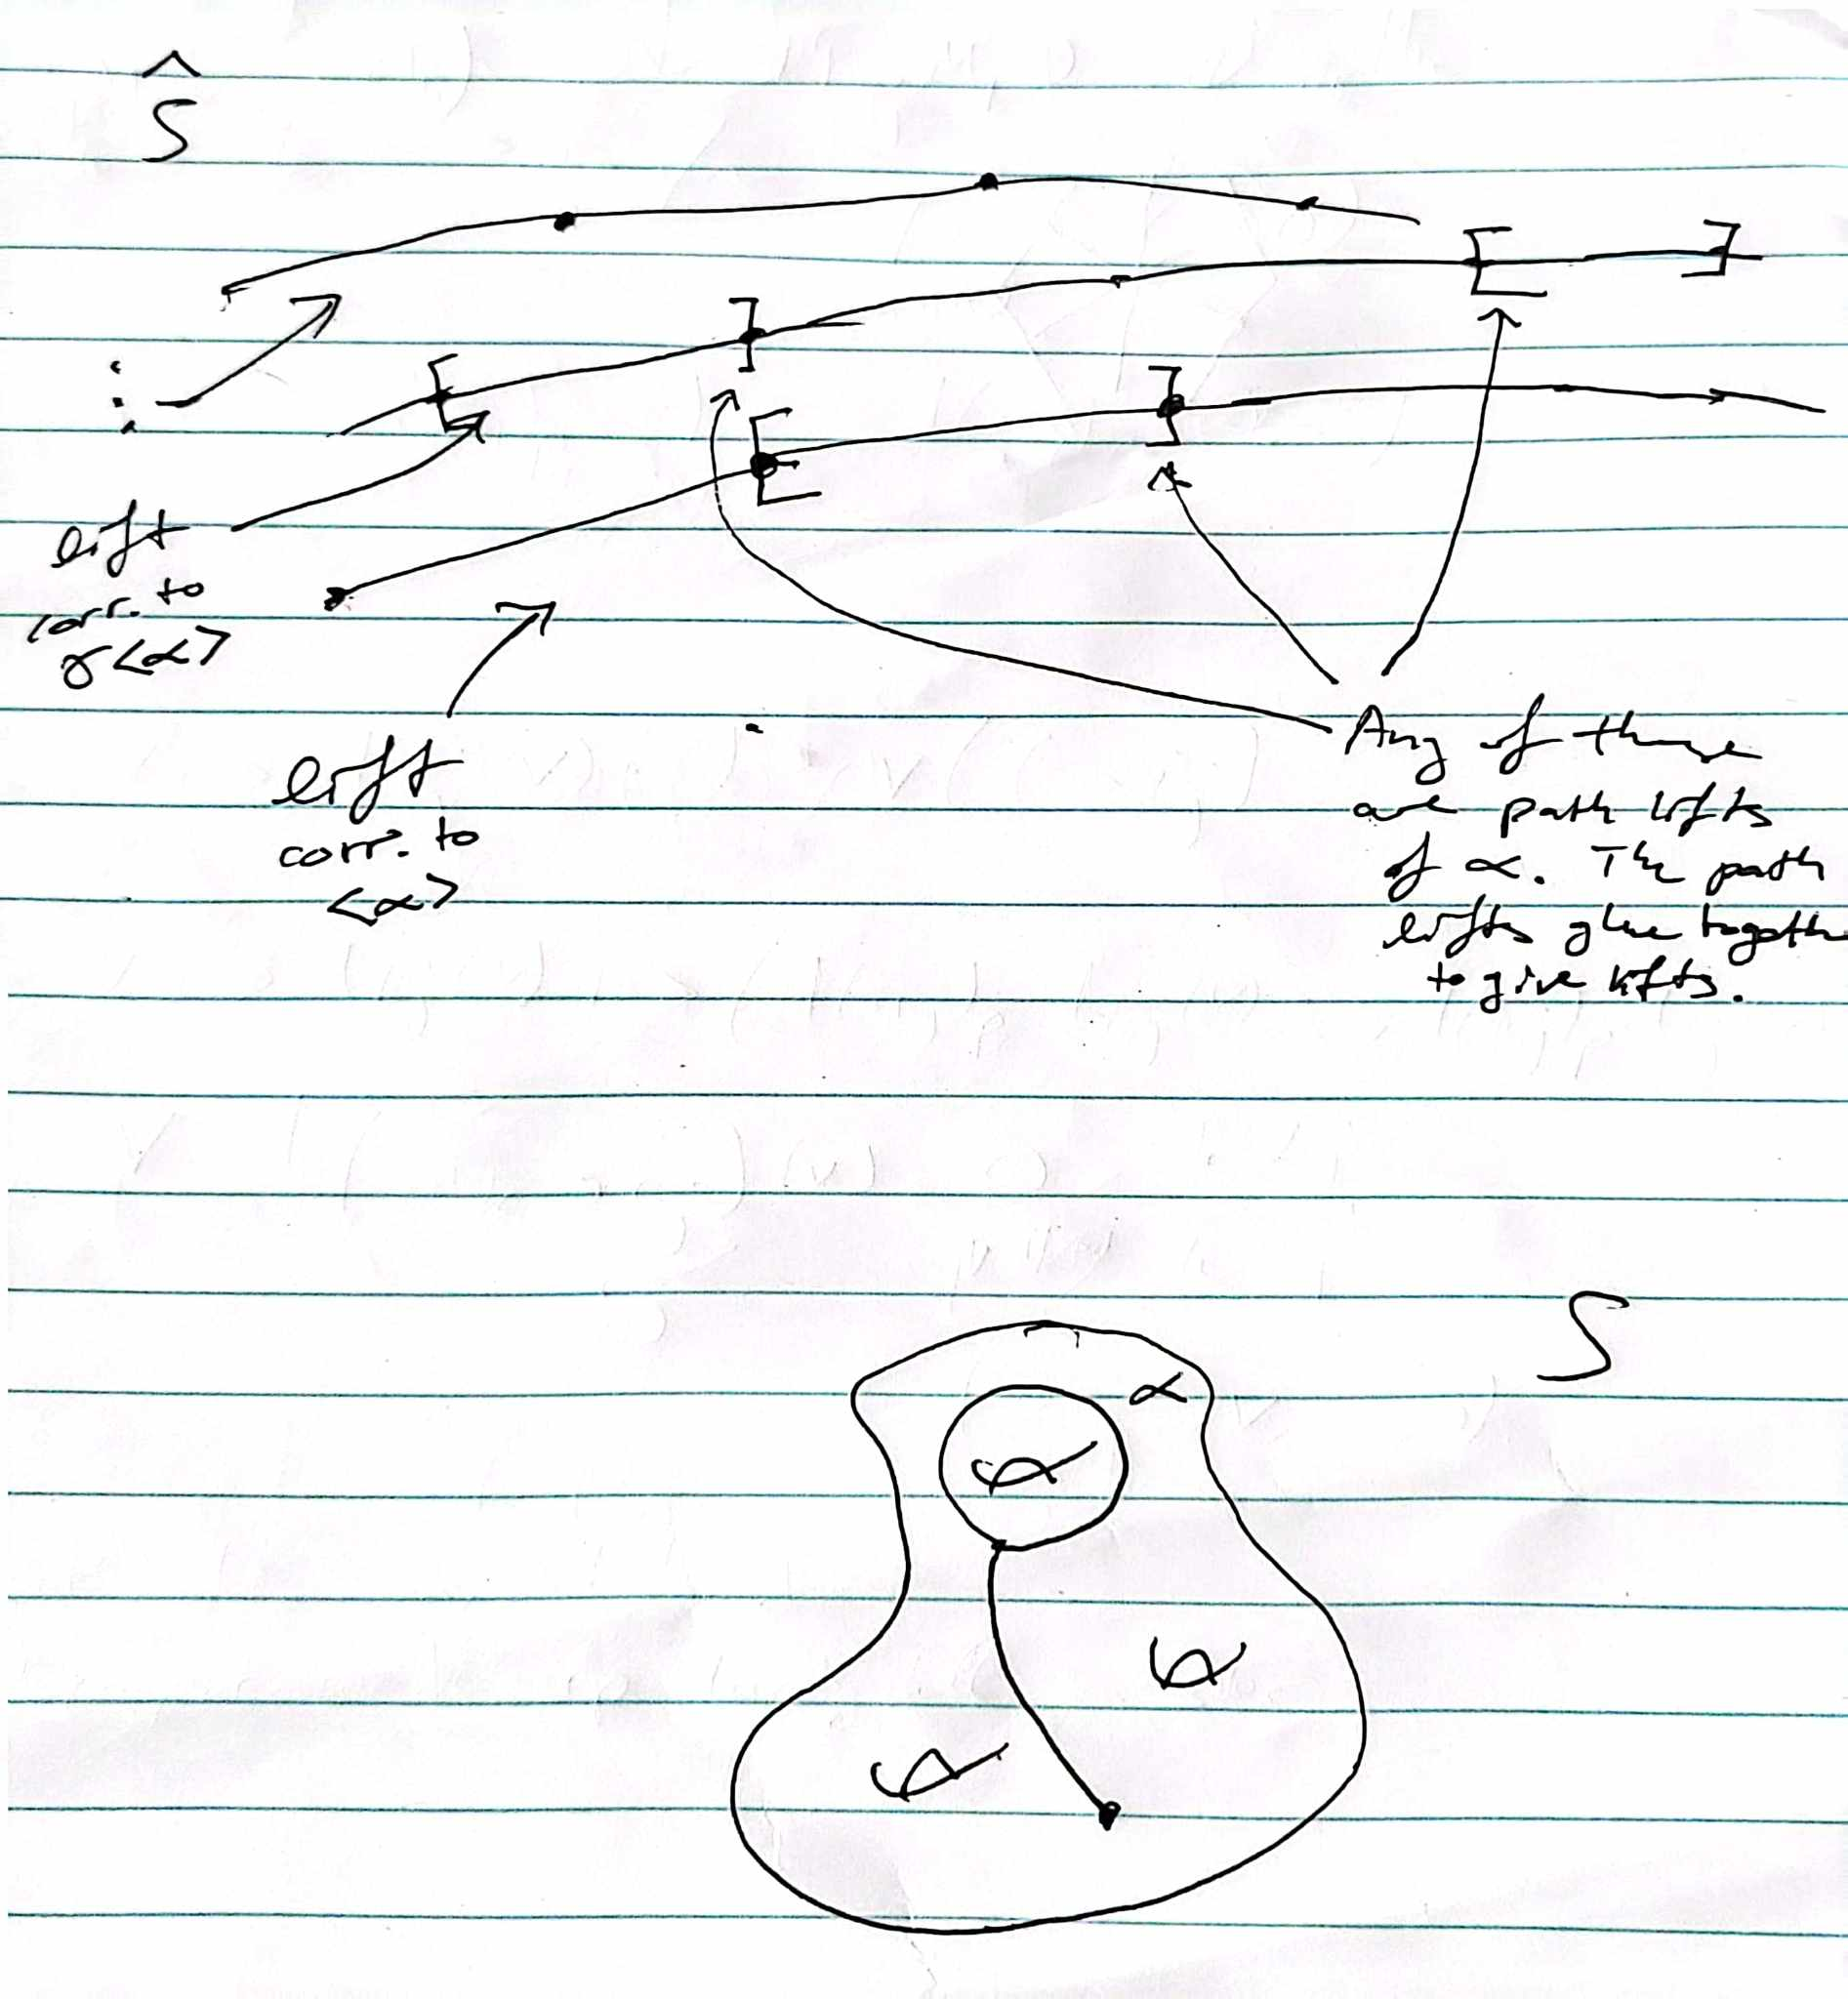
\includegraphics[width=0.8\textwidth]{lifts-of-paths.jpg}
     \caption{}
     \label{fig:lifts-of-paths}
 \end{figure}

 \begin{theorem}[]
When $S$ admits a hyperbolic metric and
$\alpha$ is a primitive element of $\pi_1 (S)$, we have
a bijective correspondence
\[
\left\{ 
    \begin{tabular}{c}
    Elements of the conjugacy\\
    class of $\alpha$ in $\pi_1 (S)$
\end{tabular}
\right\} 
\longleftrightarrow
\left\{ 
    \begin{tabular}{c}
    Lifts to $\tilde{S}$ of the\\
    closed curve $\alpha$
\end{tabular}
\right\} 
\] 


More precisely, we claim that the map which sends the lift
given by the coset $\gamma \left<\alpha \right>$ to
$\gamma \alpha \gamma^{-1}$ is bijective and well-defined.\\
 \end{theorem}

 \begin{proof}
To show that it is well-defined, suppose $\gamma \left<\alpha \right>$ and
$\beta \left<\alpha \right>$ give the same lift. Then
$\gamma = \beta \alpha^k$. So in particular,
\[
    \gamma \alpha \gamma^{-1} = \beta \alpha^k \alpha \alpha^{-k} \beta^{-1}
    = \beta \alpha \beta^{-1}
\] 
so they do correspond to the same element of the conjugacy class
$\left[ \alpha \right] $. It is clear that this is a surjective map.
Now suppose that $\gamma \alpha \gamma^{-1} = \beta \alpha \beta^{-1}$. 
Then $\beta^{-1} \gamma \alpha \left( \beta^{-1} \gamma \right)^{-1} =
\alpha$, so in particular, $\beta^{-1} \gamma \in C_{\pi_1(S)}(\alpha)$
which is a cyclic group generated by, say, $\theta$. But then
$\theta^l = \alpha$ since $\alpha$ is trivially in the centralizer of
$\alpha$; however, $\alpha$ is primitive, so
$l$ must be $\pm 1$, but then  $\alpha$ generates the centralizer of
$\alpha$, $C_{\pi_1 (S)}(\alpha) = \left<\alpha \right>$, and hence
$\gamma = \beta \alpha^l$, so $\gamma \left<\alpha \right>
= \beta \left<\alpha \right>$.
 \end{proof}

 \begin{remark}[]
     If $\alpha$ is any multiple, then we still have a bijective correspondence
     between elements of the conjugacy class of $\alpha$ and the
     lifts of $\alpha$. However, if $\alpha$ is not primitive and not
     a multiple, then there are more lifts of $\alpha$ than there
     are conjugates. Indeed, if $\alpha = \beta^{k}$, where $k > 1$, then
     $\beta \left<\alpha \right> \neq \left<\alpha \right>$ while
     $\beta \alpha \beta^{-1} = \alpha$.
 \end{remark}

 \begin{example}[]
     The above correspondence does not hold for the torus $T^2$ because
     each closed curve has infinitely many lifts, while
     each element of $\pi_1 \left( T^2 \right) \approx \mathbb{Z}^2$ 
     is its own conjugacy class because $\pi_1 \left( T^2 \right) $ is
     abelian. 
 \end{example}

 \subsubsection*{Geodesic representatives}
 \begin{proposition}[]\label{unique-geodesic-representative}
     Let $S$ be a hyperbolic surface. If $\alpha$ is a closed curve
     in $S$ that is not homotopic into a neighborhood of a puncture, then
     $\alpha$ is homotopic to a unique geodesic closed curve $\gamma$.
 \end{proposition}
 
 \begin{corollary}
     For compact hyperbolic surfaces, 
     there is a bijective correspondence:
\[
\left\{ 
    \begin{tabular}{c}
        Conjugacy classes\\
        in $\pi_1 (S)$
\end{tabular}
\right\} 
\longleftrightarrow
\left\{ 
    \begin{tabular}{c}
        Oriented geodesic\\
        closed curves in $S$
\end{tabular}
\right\} 
\] 
 \end{corollary}

 \subsection*{Simple closed curves}
 
\begin{definition}[Simple curves]
    A closed curve in $S$ is \textit{simple} if it is topologically embedded, i.e.,
    if the map $S^{1} \to S$ is injective.  
\end{definition}

By \cite[Thm~11.8]{Bredon}, any closed curve $\alpha$ can be approximated 
(arbitrarily close) by
a smooth closed curve which is homotopic to $\alpha$. Moreover,
if $\alpha$ is simple, then the smooth approximation can be chosen to be
simple. Smooth curves are advantageous because we can make use of notions
such as transversality.

Simple closed curves are also natural to study because they represent
primitive elements of $\pi_1 (S)$.

\begin{proposition}[]
    Let $\alpha$ be a simple closed curve in a surface $S$. If $\alpha$ 
    is not null homotopic, then each element of the corresponding conjugacy
    class in $\pi_1(S)$ is primitive.
\end{proposition}

\subsection*{Example: simple closed curves on the torus}

\begin{proposition}[]
    The nontrivial homotopy classes of oriented simple closed
    curves in $T^2$ are in bijective correspondence with the set of primitive
    elements of $\pi_1\left( T^2 \right) \approx \mathbb{Z}^2$ which is
    the set of elements $\left( p,q \right)  \in \mathbb{Z}^2$ such that
    either $(p,q) = (0,\pm 1)$ or  $(p,q) = (\pm 1,0)$ or
     $\gcd(p,q) = 1$.
\end{proposition}

\subsection*{Closed geodesics}

\begin{proposition}[]
    Let $S$ be a hyperbolic surface. Let $\alpha$ be a closed curve
    in $S$ not homotopic into a neighborhood of a puncture. Let
    $\gamma$ be the unique geodesic in the free homotopy class of
    $\alpha$ guaranteed by proposition \ref{unique-geodesic-representative}.
    If $\alpha$ is simple, then $\gamma$ is simple.
\end{proposition}

\begin{proof}
    Follows from the following lemma:
    \begin{lemma}[]
        Let $X$ be a topological space with a universal covering space
         $\tilde{X}$. A closed curve $\beta$ in $X$ is simple if and
        only if the following properties hold:
        \begin{enumerate}
            \item Each lift of $\beta$ to $\tilde{X}$ is simple.
            \item No two lifts of $\beta$ intersect.
            \item  $\beta$ is not a nontrivial multiple of another closed
                curve.
         \end{enumerate}
    \end{lemma}
\end{proof}

\subsection*{Intersection numbers}

It is often useful to put an inner product on a vector space to check
if two vectors are linearly independent. We can pursue something similar for
surfaces.

\begin{definition}[Geometric intersection number]
    Let $\alpha, \beta$ be closed curves on a surface $S$.
    Their \textit{geometric intersection number} is
    \[
    i \left( \alpha, \beta \right) =
    \min_{\alpha' \simeq \alpha, \beta' \simeq \beta}
    \# \left( \alpha' \cap \beta' \right) 
    \] 
\end{definition}

\begin{definition}[Preliminary definition for transversality]
If $\alpha \cap \beta$ is finite and, at every intersection, each
curve locally separates the other curve, then we say that
$\alpha$ and $\beta$ are \textit{transverse}.
\end{definition}

\begin{definition}[Minimal position]
    Two curves $\alpha$ and $\beta$ are in \textit{minimal
    position} if $\# \left( \alpha \cap \beta \right) =
    i\left( \alpha, \beta \right) $.
\end{definition}

\subsection*{Bigons}

We want a procedure to put curves into minimal position so
we can compute intersection numbers.

For this, we need the notion of a \textit{bigon}:

\begin{definition}[Bigon]
    Two transverse simple closed curves $\alpha$ and $\beta$ 
    in a surface $S$ form a \textit{bigon} if there is a
    topologically embedded disk in $S$ (the bigon) whose
    boundary is the union of an arc of $\alpha$ and an
    arc of  $\beta$ intersecting in exactly two points.
\end{definition}

\begin{figure}[http]
    \centering
    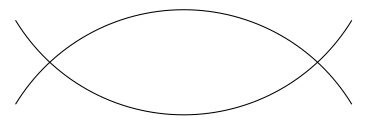
\includegraphics[width=0.4\textwidth]{bigon.png}
    \caption{Local picture of a bigon}
    \label{fig:bigon}
\end{figure}

\begin{lemma}[]\label{lemma-intersections-of-lifts}
    If transverse simple closed curves $\alpha$ and $\beta$ in
    a surface $S$ do not form any bigons, then in the
    universal cover of $S$, and pair of lifts
    $\tilde{\alpha}$ and $\tilde{\beta}$ of $\alpha$ and $\beta$ 
    intersect in at most one point.
\end{lemma}

\begin{figure}[h]
    \centering
    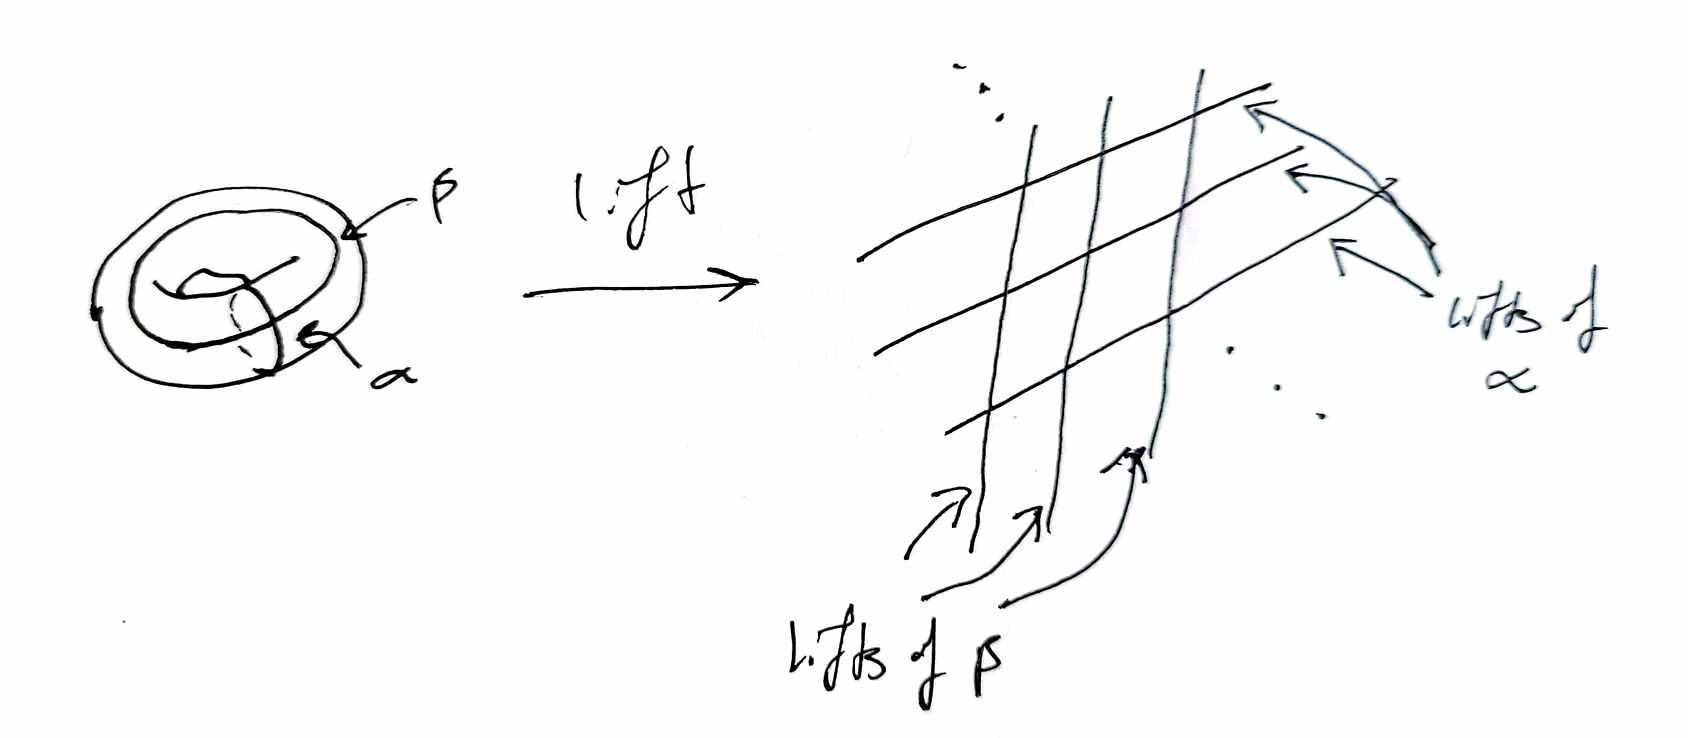
\includegraphics[width=0.8\textwidth]{lemma-1-8.jpg}
    \caption{Lemma \ref{lemma-intersections-of-lifts} illustrated}
    \label{fig:lemma-1-8-jpg}
\end{figure}


\begin{proposition}[The bigon criterion]
    Two transverse simple closed curves in a surface $S$ are in
    minimal position if and only if they do not form
    a bigon.
\end{proposition}

\begin{corollary}
    Any two transverse simple closed curves that intersect exactly once are in
    minimal position.
\end{corollary}

\subsection*{Homotopy versus isotopy for simple closed curves}

\begin{definition}[Isotopy]
    Two simple closed curves $\alpha$ and $\beta$ are \textit{isotopic}
    if there is a homotopy 
    \[
    H \colon S^{1} \times \left[ 0,1 \right] \to 
    S
    \] 
    from $\alpha$ to $\beta$ with the property that the closed
    curve $H \left( S^{1} \times \left\{ t \right\}  \right) $ 
    is simple for each $t \in \left[ 0,1 \right] $.
\end{definition}

\begin{proposition}[Baer]
    Let $\alpha$ and $\beta$ be two essential simple closed curves
    in a surface $S$. Then $\alpha$ is isotopic to $\beta$ if and
    only if $\alpha$ is homotopoic to $\beta$.
\end{proposition}

\begin{proof}
    If $\alpha$ is isotopic to $\beta$ then they are clearly also
    homotopic.\\
    \linebreak
    Suppose $\alpha$ and $\beta$ are homotopic. Taking a
    tubular neighborhood around $\alpha$, we can find
    a disjoint simple loop $\tilde{\alpha}$ which is homotopic to
    $\alpha$ but disjoint from it. Then $\beta$ is homotopic
    to $\tilde{\alpha}$, and hence
    $i \left( \alpha, \beta \right) 
    = i \left( \alpha, \tilde{\alpha} \right) = 0$.
    Performing an isotopy of $\alpha$, we may assume that
    $\alpha$ is transverse to $\beta$ (why?).
    If $\alpha$ and $\beta$ are not disjoint, then by
    the bigon criterion, they form a bigon. A bigon
    prescribes an isotopy that reduces intersection, so we
    may remove bigons by isotopy until $\alpha$ and $\beta$ are
    disjoint.\\
    \linebreak
    Suppose $\chi (S) <0$. Lift $\alpha$ and $\beta$ to
    $\tilde{a}$ and $\tilde{\beta}$ with the
    same endpoints in $\partial \mathbb{H}^2$. There
    is a hyperbolic isometry $\varphi$ that leaves
    $\tilde{\alpha}$ and $\tilde{\beta}$ invariant and
    acts by translation on the lifts. As $\tilde{\alpha}$ and
    $\tilde{\beta}$ are disjoint, let $R$ denote the region
    between them. We claim that the quotient surface
    $R' = R / \left<\varphi \right>$ is an annulus.
    The fundamental group of $R'$ is isomorphic to the group of
    deck transformations $\left<\varphi \right>$ and is hence
    infinite cyclic. Furthermore, $R'$ has two boundary components.
\end{proof}


\subsubsection*{Extension of isotopies}

\begin{definition}[]
    An isotopy of a surface $S$ is a homotopy $H \colon 
    S \times I \to S$ such that for each
    $t \in \left[ 0,1 \right] $, the map
    $H \left( S, t \right) \colon S \times \left\{ t \right\} \to 
    S$ is a homeomorphism. Given an isotopy between
    two simple closed curves in $S$, it will often be useful
    to promote this to an isotopy of $S$ which we call an
    ambient isotopy of $S$.
\end{definition}

\begin{proposition}[]
    Let $S$ be any surface. If $F \colon S^{1} \times I \to 
    S$ is a smooth isotopy of simple closed curves, then
    there is an isotopy $H \colon S \times I \to S$ so that
    $H |_{S \times 0}$ is the identity and 
    $H|_{F\left( S^{1} \times 0 \right) \times I} = F$.
\end{proposition}

\begin{proof}
    \cite[Ch~8, Thm 1.3]{Hirsch}
\end{proof}

\subsection{Small digression on Hirsch chapter 8}

\begin{definition}[Isotopy in general and their tracks]
    Let $V$ and $M$ be manifolds. An
    isotopy from $V$ to $M$ is a map
    $F \colon V \times I \to M$ such that
    for each $t \in I$, the map
    \[
    F_t \colon V \to M, \quad x \mapsto F(x,t)
    \] 
    is an embedding.

    The \textit{track} of the isotopy $F$ is the embedding
    \[
    \hat{F} \colon V \times I \to M \times I, \quad
    \left( x,t \right) \mapsto \left( F(x,t),t \right) 
    \] 
\end{definition}

\begin{definition}[Isotopic embeddings and ambient isotopies]
    If $F \colon V \times I \to M$ is an isotopy, we call
    the two embeddings $F_0$ and $F_1$ 
    isotopic. If $V$ is a submanifold of $M$ and
    $F_0$ is the inclusion, we call $F$ an isotopy
    of $V$ in $M$.
    When $V = M$ and each $F_t$ is a diffeomorphism, and
    $F_0 = \mathbbm{1}_M$, then $F$ is called
    an ambient isotopy.
\end{definition}

\begin{definition}[Support of isotopy]
    The \textit{support} $\Supp F
    \subset V $ of an isotopy $F \colon V \times I \to M$ 
    is the closure of
    $\left\{ x \in V \colon
    F(x,t) \neq F(x,0) \text{ for some }
t \in I\right\} $.
\end{definition}


\begin{theorem}[Isotopy extension theorem]\label{Hirsch-isotopy-extension}
    Let $V \subset M$ be a compact submanifold
    and $F \colon V \times I \to M$ an isotopy
    of $V$. If either $F\left( V \times I \right) 
    \subset \partial M$ or $F\left( V \times I \right) 
    \subset M - \partial M$, then $F$ extends to
    an ambient isotopy of $M$ having compact support.
\end{theorem}




\subsection*{Arcs}
$ $ \newline \newline
Assume $S$ is a compact surface, possibly with boundary
and possibly with finitely many marked points in the interior.
Denote the set of marked points by $\mathcal{P}$.

\begin{definition}[]
    A \textit{proper arc} in $S$ is a map $\alpha \colon
    \left[ 0,1 \right]  \to S$ such that
    $\alpha^{-1} \left( \mathcal{P} \cup \partial S \right) 
    = \left\{ 0,1 \right\} $.
\end{definition}
\begin{definition}[]
    The arc $\alpha$ is \textit{simple} if it is an embedding
on its interior.
\end{definition}

\begin{remark}[]
    The homotopy class of a proper arc is taken to be
    the homotopy class within the class of proper arcs.
    Thus points on $\partial S$ cannot move off the boundary
    during the homotopy.\\
    A homotopy (or isotopy) of an arc is said to
    be \textit{relative to the boundary} if its endpoints
    stay fixed throughout the homotopy. 
    An arc in a surface $S$ is \textit{essential} if it
    is neither homotopic into a boundary component of $S$ nor a
    marked point of $S$.
\end{remark}

\begin{figure}[htpb]
    \centering
    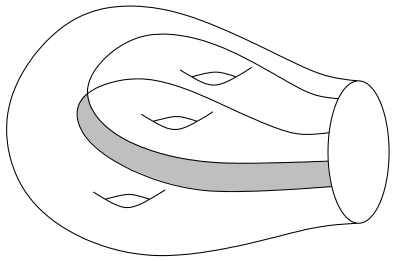
\includegraphics[width=0.5\textwidth]{bigon-of-arcs.png}
    \caption{bigon-of-arcs.png}
    \label{fig:bigon-of-arcs-png}
\end{figure}
Note in this picture how if isotopies are considered relative
to the boundary, then the two arcs are in minimal position, while
if we consider general isotopies, then the half-bigon shows that
they are not in minimal position as we can pull the top strand down
under the bottom one along the boundary.

\begin{itemize}
    \item The bigon criterion holds for arcs.
    \item Corollary 1.9 (geodesics are in minimal position)
        and prop 1.3 (existence and uniqueness of geodesic 
        representatives) work for arcs in surfaces with
        punctures and/or boundary.
    \item Prop 1.10 (homotopy versus isotopy for curves) and
        theorem 1.13 (extension of isotopies) also
        work for arcs.
\end{itemize}

\subsection*{Change of coordinates principle}

\subsubsection*{Classification of simple closed curves}

\begin{definition}[]
    Given a simple closed curve or
    a simple proper arc $\alpha$ in a surface $S$,
    the surface obtain by cutting $S$ along $\alpha$ is
    a compact surface $S_{\alpha}$ equipped with an attaching
    map $h$ (i.e.
    \begin{enumerate}
        \item $S_{\alpha} / \left( x \sim h(x) \right) 
            \approx S$ 
        \item the image of the distinguished boundary components
            under this quotient map is $\alpha$.
    \end{enumerate}
\end{definition}

\begin{definition}[]
    We say that a simple closed curve $\alpha$ in the surface
    $S$ is \textit{nonseparating} if the cut surface
    $S_{\alpha}$ is connected, and \textit{separating} if
    $S_{\alpha}$ is not connected.
\end{definition}


\begin{theorem}[]
    If $\alpha$ and $\beta$ are any two nonseparating simple
    closed curves in a surface $S$, then there
    is a homeomorphism $\varphi \colon S \to S$ with
    $\varphi \left( \alpha \right) = \beta$.
\end{theorem}

\begin{proof}
    The cut surface $S_{\alpha}$ and $S_{\beta}$ have
    two boundary component corresponding to $\alpha$ and 
    $\beta$, respectively. 
    Now, suppose $S_{\alpha}$ has
    $n_{\alpha}$ vertices, $m_{\alpha}$ edges and
    $t_{\alpha}$ triangles in a triangulation. Then
    in obtaining $S$ from $S_{\alpha}$, we identify the vertices
    and edges, but no triangles are identified, so we get
    $n_{S} = n_{\alpha}-3$ and $m_{S} = m_{\alpha}-3$, but
    $t_{S} = t_{\alpha}$. Thus $\chi (S_{\alpha}) = 
    \chi (S)$.

    Since both $S_{\alpha}$ and
    $S_{\beta}$ have the same Euler characteristic, number of
    boundary components and number of punctures, it follows
    that $S_{\alpha} \approx S_{\beta}$. Choose
    a homeomorphism $\varphi \colon S_{\alpha} \to S_{\beta}$ such 
    that if $h_{\alpha}$ is the attaching map for $S_{\alpha}$ 
    and $h_{\beta}$ is the attaching map for $S_{\beta}$,
    then $\varphi$ takes $\left\{ x, h_{\alpha}(x) \right\} $ 
    to $\left\{ y, h_{\beta}(y) \right\} $ - i.e., the
    identification are respected under the map.
    This homeomorphism gives the desired
    homeomorphism of $S$ taking $\alpha$ to $\beta$.
    If we want an orientation preserving homeomorphism, we
    can postcompose by an orientation-reversing homeomorphism
    fixing $\beta$ if necessary.
\end{proof}

\begin{theorem}[]
    When $S$ is closed, $\beta$ is separating if and only
    if it is the boundary of some subsurface of $S$. Which
    is equivalent to the vanishing of the
    homology class of $\beta$ in $H_1 \left( S, \mathbb{Z} \right) $.
\end{theorem}

\begin{remark}[]
    By the "classification of disconnected surfaces", there
    are finitely many separating simple closed curves in $S$ 
    up to homeomorphism.
\end{remark}


\begin{corollary}\label{cut-surface-homeo-1}
    There is an orientation-preserving homeomorphism of a surface
    taking one simple closed curve to another if and only
    if the corresponding cut surfaces (which may be disconnected)
    are homeomorphic.
\end{corollary}

\begin{definition}[Topological type]
    The existence of a homeomorphism as in \ref{cut-surface-homeo-1}
    is an equivalence relation. The equivalence class
    of a simple closed curve or a collection of simple closed
    curves is called its \textit{topological type}.
\end{definition}

A seprarating simple closed curve in the closed surface
$S_g$ divides $S_g$ into two disjoint subsurfaces of genus
$k$ and $g-k$. The minimum of $\left\{ k, g-k \right\} $ is
called the genus of the separating simple closed curve. 
There are $\left\lfloor \frac{g}{2} \right\rfloor$ topological
types of essential separating simple closed curves in
a closed surface.

\begin{question}
    Suppose $\alpha$ is any nonseparating simple closed curve
    on a surface $S$.
    \begin{enumerate}
        \item Is there a simple closed curve
            $\gamma$ in $S$ so that $\alpha$ and $\gamma$ 
            \textit{fill} $S$, i.e., such that
            $\alpha$ and $\gamma$ are in minimal position
            and the complement of $\alpha \cup  \gamma$ is
            a union of topological disks.
        \item Is there a simple closed curve $\delta$ in
            $S$ with $i(\alpha,\beta) = 0$? $i(\alpha,\beta)=1$?
            $i(\alpha,\beta)=k$?
    \end{enumerate}
\end{question}

\begin{figure}[htpb]
    \centering
    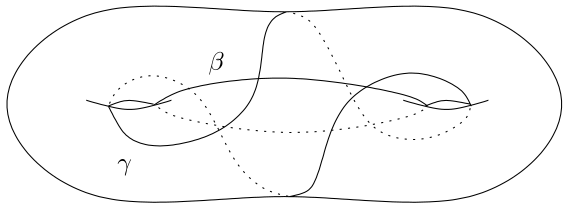
\includegraphics[width=0.7\textwidth]{filling-genus-2-surface.png}
    \caption{a}
    \label{fig:filling-genus-2-surface-png}
\end{figure}

Figure \ref{fig:filling-genus-2-surface.png} shows
two filling simple closed curves on the genus $2$ surface.
By the classification of simple closed curves on a surface,
there is a homeomorphism $\varphi \colon S_2 \to S_2$ such
that $\varphi\left( \beta \right) =\alpha$. Then
the image of $\gamma$ under $\varphi$ fills $S_2$ with
$\alpha$ since filling is a topological property (show this).

\subsubsection*{Examples of change of coordinate principle}

\begin{enumerate}
    \item \textit{Pairs of simple closed curves that intersect
        once are all of the same topological type}.
        Suppose $\alpha_1$ and $\beta_1$ form
        such a pair on a surface $S$. Then
        $\beta_1$ must be an arc connecting the two
        boundary components in $S_{\alpha_1}$. But the boundary
        component is homeomorphic to $S^{1}$, so removing a 
        point leaves it connected. Thus removing
        $\beta_1$ leaves $\left( S_{\alpha_1} \right)_{\beta_1}$
        path-connected. Similarly,
        $\left( S_{\alpha_2} \right)_{\beta_2}$ is path-connected
        for any other pair $\alpha_2$ and $\beta_2$ that
        constitute a pair of simple closed curves
        that intersect once in $S$. By the classification
        of surfaces with boundary, $\left( S_{\alpha_1} \right)_{\beta_1}$ is
        homeomorphic to $\left( S_{\alpha_2} \right)_{\beta_2}$ 
        which preserves equivalence classes on the boundary,
        and as we can construct this homeomorphism first
        for the $\beta$'s and then for the $\alpha$'s, 
        this homeomorphism descends to a self-homeomorphism
        of $S$ taking the pair $\left\{ \alpha_1, \beta_1 \right\} $ 
        to $\left\{ \alpha_2, \beta_2 \right\} $.
\end{enumerate}


\subsection*{Three facts about homeomorphisms}

Suppose $f \colon D \to D$ is an orientation-reversing map.
Then $f$ restricts to a map on $S^{1} \to S^{1}$, and
if $f$ is smooth considered as such a map, then the
reversal of orientation implies that since the fiber
of any point is a single point, the degree of $f$ 
must be $-1$. But thus $f$ is not isotopic to the identity
as the identity has degree $1$ and the isotopy would
have to restrict to a homotopy on the boundary, but
degree is a homotopy invariant for maps $S^{n} \to S^{n}$.\\
However, the straight-line homotopy does give a homotopy
between $f$ and the identity.\\
\linebreak
On $A = S^{1} \times I$, the orientation-reversing map
that fixes the $S^{1}$ factor and reflects the $I$ factor
is homotopic but not isotopic to the identity.


\begin{theorem}[]
    Let $S$ be any compact surface and let $f$ and $g$ be
    homotopic homeomorphisms of $S$. Then $f$ and $g$ are
    isotopic unless they are one of the two examples described
    above (on $S = D^2$ and $S = A$ ). In particular,
    if $f$ and $g$ are orientation-preserving, then they
    are isotopic.
\end{theorem}



\begin{theorem}[]
    Let $S$ be a compact surface. Then every homeomorphism of
    $S$ is isotopic to a diffeomorphism of $S$.
\end{theorem}

\begin{theorem}[Hamstrom]
    Let $S$ be a compact surface, possibly minus a finite
    number of points from the interior. Assume that
    $S$ is not homeomorphic to
    $S^2, \mathbb{R}^2, D^2, T^2$, the closed annulus,
    the once-punctured disk, or the once-punctured plane. Then
    the space $\Homeo_0 (S)$ is contractible.
\end{theorem}




\newpage

\section{Mapping class group basics}


\subsection*{The compact-open topology}

\begin{definition}[]
    The \textit{weak} or \textit{compact-open $C^{r}$ }
    topology on $C^{r} \left( M,N \right) $, where
    $M$ and $N$ are $C^{r}$ manifolds, is generated
    by sets defined as follows:
    let $f \in C^{r}(M,N)$. Let $\left( U, \varphi \right),
    \left( V, \psi  \right) $ be charts on
    $M$ and $N$ ; let $K \subset U$ be compact such that
    $f(K) \subset V$ and let $0 < \varepsilon \le 
    \infty $. Then a \textit{weak subbasic neighborhood}
    \[
    \mathcal{N}^{r} \left( f ; \left( U, \varphi  \right) ,
    \left( V, \psi  \right) , K, \varepsilon \right) 
    \tag{$\zeta$}\label{eq:compact-open-subbasis-nbhds}
    \] 
    is the set of $C^{r}$ maps $g \colon M \to N$ such that
    $g(K) \subset V$ and
    \[
    \|D^{k}\left( \psi f \varphi^{-1} \right) (x)
    -D^{k} \left( \psi g \varphi^{-1} \right) (x)\|< \varepsilon
    \] 
    for all $x \in \varphi(K)$, for $k = 0, \ldots, r$.
    The \textit{compact-open $C^{r}$ topology} on
    $C^{r}(M,N)$ is generated by the set of weak subbasic
    neighborhoods, and defines the topological space
    $C_W^{r} (M,N)$.
    A neighborhood of $f$ is then
    any set containing the intersection
    of a finite number of sets of the
    type \eqref{eq:compact-open-subbasis-nbhds}.
\end{definition}

We are interested in the subspace
$\Homeo (S) \subset C_W^{0} (S,S)$, inheriting the
subspace topology.\\
\linebreak
The compact-open topology might seem a bit confusing, but
we have the following lemma \cite[Prop A.14]{Hatcher}:

\begin{lemma}[]\label{compact-open-isotopy}
    Let $X,Y,Z$ be Hausdorff topological spaces.
    Suppose $Y$ is locally compact. Then a 
    map $f \colon X \to C_W^{0}(Y,Z)$ is
    continuous if and only if the associated map
    $F \colon X \times Y \to Z$ defined by
    \[
    F(x,y) := f(x)(y)
    \] 
    is continuous.
\end{lemma}





\subsection{Definitions and first examples}

\begin{definition}[]
    Let $S$ be a surface which is the connected sum of $g\ge 0$ 
    tori with $b \ge 0$ disjoint open disks removed and
    $n \ge 0$ points removed from the interior. Let
    $\Homeo^{+} \left( S, \partial S \right)$ denote the group
    of orientation-preserving homeomorphisms of $S$ that
    restrict to the identity on $\partial S$. We endow this
    group with the compact-open topology.
    The \textit{mapping class group} of  $S$, denoted
    $\Mod (S)$, is the group
    \[
    \Mod(S) = \pi_0 \left( \Homeo^{+} \left( S, \partial S
    \right) \right) 
    \] 


\begin{remark}[]
    From Lemma \ref{compact-open-isotopy}, we
    see that a path $\gamma \colon I \to 
    \Homeo^{+}\left( S, \partial S \right) $
    is precisely equivalent to an isotopy 
    $F \colon I \times S \to S$ from
    $\gamma(0)$ to $\gamma(1)$ (isotopy because at each
    time $t$, $\gamma(t) \colon S \to S$ is indeed a topological
    embedding as it is a homeomorphism). In fact, it's an isotopy
    of $S$. Here isotopies are required to fix
    boundaries.
\end{remark}





    If
    $\Homeo_0 (S, \partial S)$ denotes the connected component of
    the identity in $\Homeo^{+}\left( S, \partial S \right) $, then
    we can equivalently write
    \[
    \Mod (S) = \Homeo^{+} \left( S, \partial S \right) /
    \Homeo_0 \left( S, \partial S \right) .
    \] 
\end{definition}

\begin{proposition}[]
    \begin{align*}
        \Mod (S) 
        &= \pi_0 \left( \Homeo^{+} \left( S, \partial S \right) 
        \right) \\
        &\approx \Homeo^{+}\left( S, \partial S \right) /
        \text{homotopy}\\
        &\approx \pi_0 \left( \mathrm{Diff}^{+} \left( 
        S, \partial S \right)  \right) \\
        &\approx \textrm{Diff}^{+}\left( S, \partial S \right) /
        \sim
    \end{align*}
    where $\mathrm{Diff}^{+}\left( S, \partial S \right) $ is the group of
    orientation preserving diffeomorphisms of $S$ that are the
    identity on the boundary and $\sim$ can be taken to be either
    smooth homotopy relative to the boundary or smooth isotopy relative to the
    boundary.
\end{proposition}

\subsubsection*{The Alexander Lemma}

\begin{lemma}[Alexander lemma]
   The group $\Mod\left( D^2 \right) $ is trivial. 
\end{lemma}

\begin{remark}
    Also $0 \approx \Mod\left( D - \left\{ 0 \right\}  \right) 
    \approx \Mod \left( S_{0,1} \right) \approx
    \Mod\left( S^2 \right) $.
\end{remark}

\subsubsection*{The mapping class group of the thrice-punctured sphere,
$\Mod \left( S_{0,3} \right) $}

\begin{proposition}[]
    Any two essential simple proper arcs in $S_{0,3}$ with the
    same endpoints are isotopic. Any two essential arcs that both
    start and end at the same marked point of $S_{0,3}$ are isotopic.
\end{proposition}

\begin{proof}
    Let $\alpha$ and $\beta$ be two simple proper arcs in
    $S_{0,3}$ connecting the same two distinct marked points.
    By isotopy, we may modify $\alpha$ so that
    it intersects transversally with $\beta$.
    Letting the last marked point become the point at infinity,
    we can consider $\alpha$ and $\beta$ as being
    arcs in $\mathbb{R}^2 - \left\{ p,q \right\} $ for
    the two marked points $p,q$.
    An example is illustrated below.
    Now, suppose the arcs are disjoint.
    Then, choosing an intersection point, we can follow
    the path to the other intersection point and obtain
    either a bigon, in which case we can remove it by isotopy,
    or a bigon with path segments inside.
    Now, suppose
    the there is some point of $\alpha$ inside the bigon.
    Then since this is part of the arc $\alpha$, we can find
    a simple path connecting this point to two points
    of $\beta$. There could, however, be infinitely many
    such paths inside the bigon, preventing us choosing the
    innermost (think concentric semicircles).
    However, by transversality, the preimages of the 
    intersection points
    form a $0$-dimensional submanifold of $I$ which is closed
    (as the preimage of a closed path segment of $ \beta$)
    and discrete.
    But discrete subsets of compact spaces are finite. Hence
    we can choose the innermost such path of $ \alpha$.
    By isotopy, we can remove the bigon formed by  this alpha.
    Continuing a finite amount of times, we remove the original
    bigon. After a finite amount of reiterations, we can
    therefore remove all bigons, and we get
    disjoint $ \alpha$ and $\beta$.

    Now suppose we remove $\alpha \cup  \beta$. Then
    we get a disjoint union of a disk and a punctured
    disk (by the classification of surfaces - expound on this).
    Thus the embedded disk in $S_{0,3}$ gives an isotopy
    of $\alpha$ to $\beta$.
\end{proof}
 



\begin{proposition}[]
    The natural map
    \[
    \Mod\left( S_{0,3} \right) \to \Sigma_{3}
    \] 
    given by the action of $\Mod\left( S_{0,3} \right) $ on the
    set of marked points of $S_{0,3}$ is an isomorphism.
\end{proposition}

\begin{proof}
    This is just additional notes to the proof in the book.
    The reason it is surjective is that the previous proposition
    gives an isotopy between arcs which we can extend to
    an ambient isotopy relative to the boundary which
    is an element of the mapping class group. (can we
    be sure the last marked point stays fixed?)
\end{proof}




\begin{exercise}[]
    Show similarly that $\Mod \left( S_{0,2} \right) \approx
    \mathbb{Z}/ 2\mathbb{Z}$.
\end{exercise}


\begin{solution}
    Let $\alpha, \beta$ be arcs with the same distinct
    marked endpoints. Equivalently to before, we can reduce
    bigons by isotopy until $\alpha$ and $\beta$ are disjoint.
    Then removing $\alpha \cup  \beta$ we would get
    two disjoint disks (firstly, $\alpha \cup \beta$ 
    make up a closed simple curve which is trivial since
    $H_1 \left( S^{1} \right) = \left\{ 0 \right\} $ and
    thus separating. Therefore we get a disconnected
    space with as many vertices as edges whose
    Euler characteristic must add to
    $2 = \chi \left( S^{2} \right) $, so
    it must precisely have $1$ face each, i.e., they are disks)
    which will descend to give the desired
    isotopy in $S_{0,2}$.
    
    So assume no intersection. Let $\varphi$ be an orientation
    preserving homeomorphism fixing the marked points. Then
     $\varphi \left( \alpha \right) $ is isotopic
     to $\alpha$, so $\varphi$ is isotopic to a homeomorphism which
     fixes $\alpha$ pointwise, call it $\psi$.
     This induces a homeomorphism on $S^{2} - \alpha$ which
     is a disk that is the identity on the boundary, and hence
     isotopic to the identity homeomorphism on the disk
     since $\Mod \left( D^2 \right) \approx \left\{ 0 \right\} $.
     This isotopy gives an isotopy of $ \psi$ to the identity.
     The composition of all these
     isotopies gives an isotopy of 
     $\varphi$ with the identity.
     Hence the map is injective.
\end{solution}



\begin{theorem}[]\label{mcg-of-torus}
    The homomorphism
    \[
    \sigma \colon \Mod \left( T^2 \right) \to 
    \SL \left( 2, \mathbb{Z} \right) 
    \] 
    given by the action on $H_1 \left( T ;\mathbb{Z} \right) 
    \approx \mathbb{Z}^2$ is an isomorphism.
\end{theorem}

\begin{proof}
    Additional notes on the proof:
    why can we for any element $f \in \Mod \left( T^2 \right) $ 
    choose a representative $\varphi $ that fixes a basepoint
    for $T^2$?
\end{proof}


\begin{corollary}
    Since $H_1 \left( S_{1,1}; \mathbb{Z} \right) \approx
    \mathbb{Z}^2$, there is a homomorphism
    $\sigma \colon \Mod \left( S_{1,1} \right) \to 
    SL(2, \mathbb{Z})$ which is determined
    which isomorphism the homomorphism induces in
    homology. This map is an isomorphism.
\end{corollary}

\begin{exercise}[]
    Prove this explicitly.
\end{exercise}

\subsubsection*{The mapping class group of
$S_{0,4}$}

Consider the torus $T^2$ as $I^2 / \sim$ under the usual
identification. Then consider the
linear map $\iota \colon \mathbb{R} \to \mathbb{R}$ 
by
$\iota = \begin{pmatrix} -1 & 0\\ 0 & -1 \end{pmatrix} 
= - I
\in SL(2, \mathbb{Z})$ which rotates about the origin
by $\pi$ radians.

The map is equivarient with respect to the quotient map
so it induces a map $I^2 / \sim \to I^2 / \sim$
and we wish to take the quotient space that identifies
fibers of this map. This is equivalent to taking
the quotient space of $\mathbb{R}^2$ induced by the
following actions: for $\left( a,b \right) \in \mathbb{R}^2$,
\begin{enumerate}
    \item sending $(a,b)$ to $(a+2k,b)$ for $k \in \mathbb{Z}$,
    \item sending $(a,b)$ to $(a, b+ 2t)$ for $t \in \mathbb{Z}$,
    \item or sending $(a,b)$ to $(-a, -b)$.
\end{enumerate}
We claim the quotient of $\left[ 0,2 \right] \times I $ 
under this action
is a fundamental domain for the action.
Clearly, the action is transitive. Now
if $(a,b),(c,d) \in (0,2) \times I $ are in the same orbit,
then
\begin{align*}
    a &= (-1)^{\alpha} c + 2k \\
    b &= (-1)^{\alpha} d + 2t
\end{align*}
for some $k,t \in \mathbb{Z}$. But then
if $b+d = 2t$, we  get $b+d \in 2 \mathbb{Z} \cap \left( 0,2 \right) 
= \varnothing$, so $\alpha$ must be even, and
$b = d$. But then
$a-c \in  2\mathbb{Z} \cap \left( -2, 2 \right) =
\left\{ 0 \right\} $, so $a=c$ and $b=d$.
The identifications on the boundary become as in figure
\ref{fig:involution-on-torus-quotient} which becomes
$S^2$.


\begin{figure}[htpb]
    \centering
    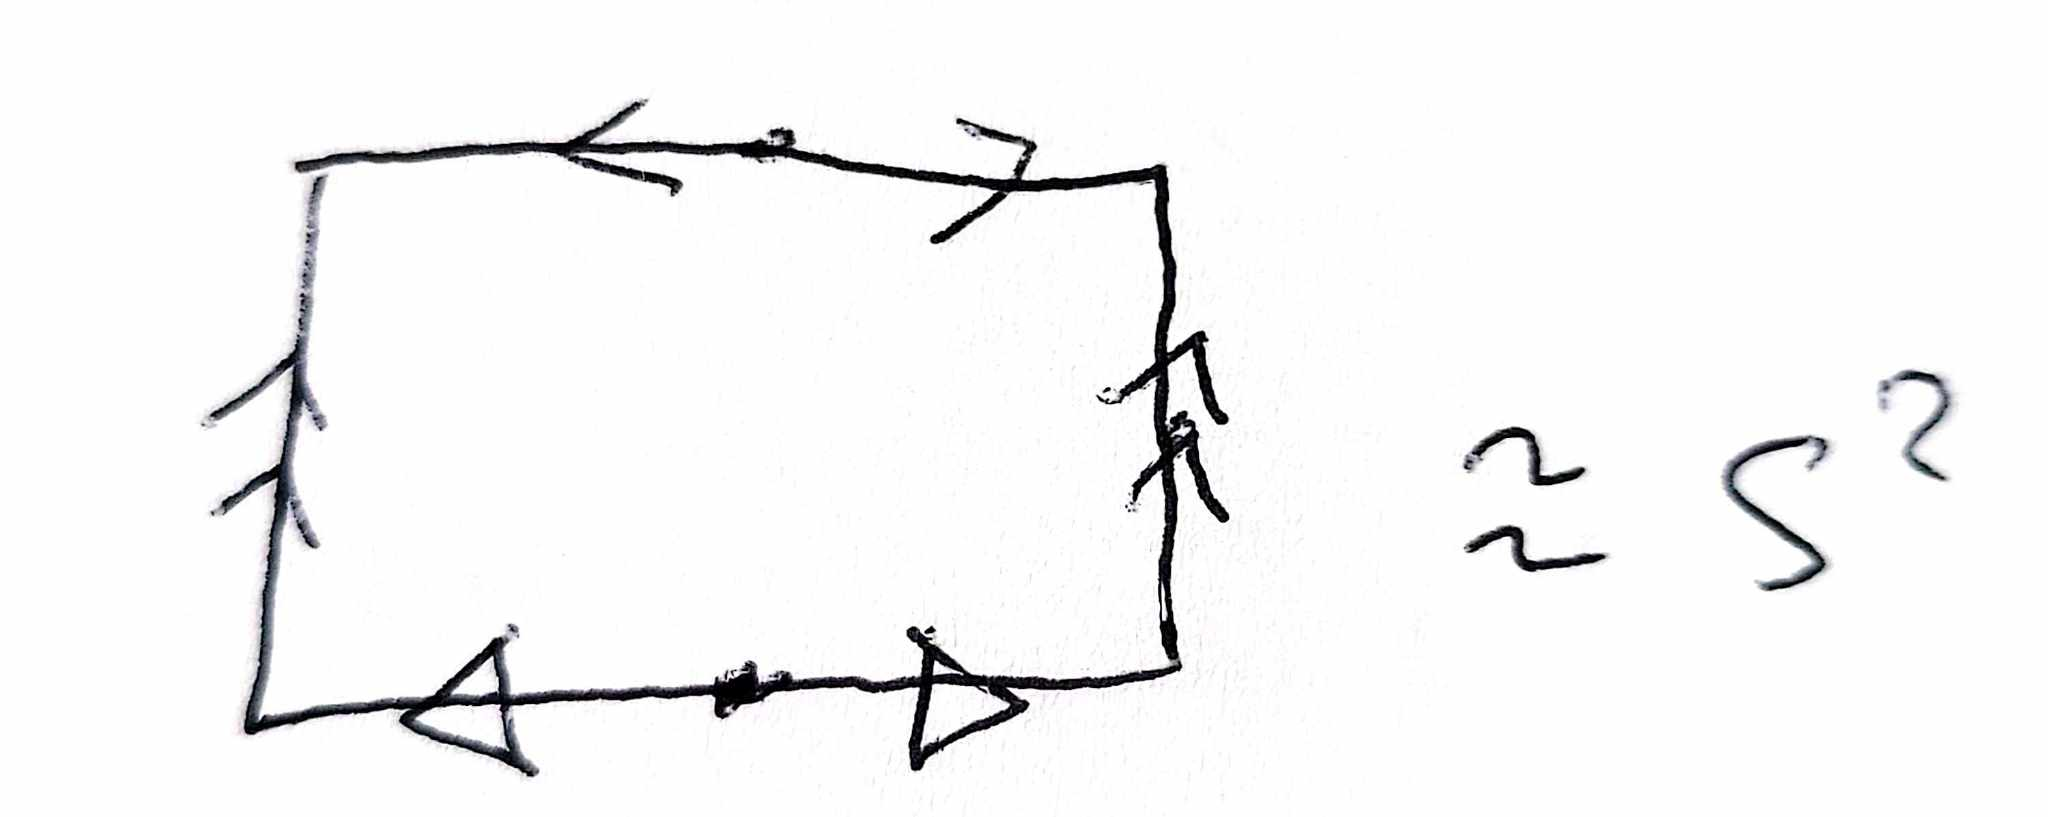
\includegraphics[width=0.6\textwidth]{involution-on-torus-quotient.jpg}
    \caption{}
    \label{fig:involution-on-torus-quotient}
\end{figure}

We identify the quotient
by $S_{0,4}$ where the $4$ marked points are
the $4$ fixed points under the involution, namely, the images
of the
center of $I^2$, the midpoints of the edges and corner vertices.
This is clearly also a $2$-fold cover of the sphere.

Now, since for any $A \in \SL (2,\mathbb{Z})$,
$A (-I) = (-I) A$,
each element of $\Mod \left( T^2 \right) $ induces
an element of $\Mod \left( S_{0,4} \right) $ by
descending to the quotient.


\begin{proposition}[]
    The hyperelliptic involution induces a bijection
    between the set of homotopy classes of essential
    simple closed curves in $T^2$ and the
    set of homotopy classes of essential simple closed 
    curves in $S_{0,4}$.
\end{proposition}

\begin{proof}
    Notes:

    \begin{figure}[htpb]
        \centering
        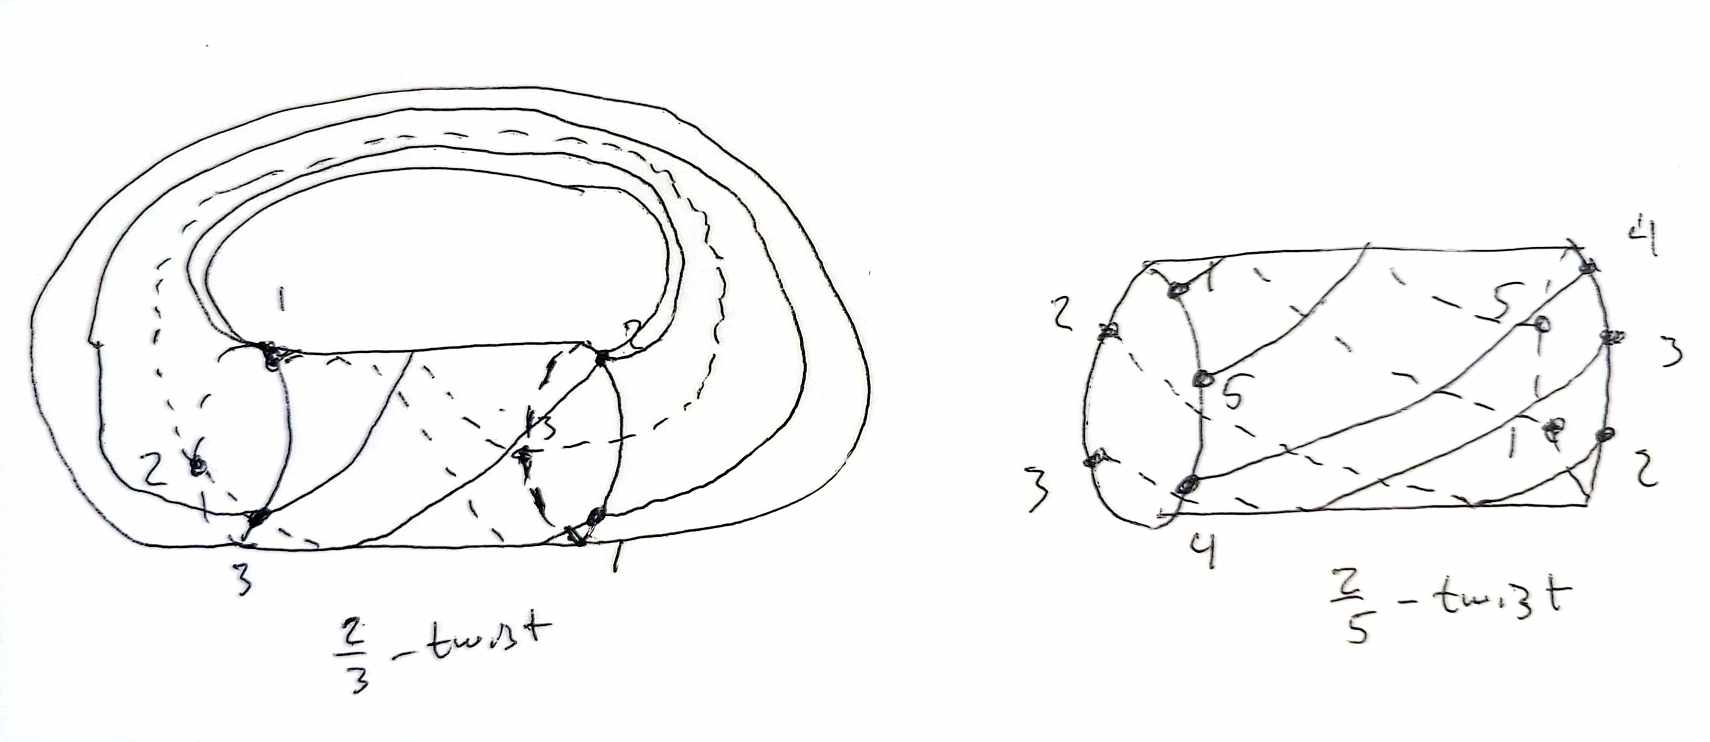
\includegraphics[width=0.9\textwidth]{twists-along-curves-on-torus.jpg}
        \caption{Twists along the meridian circle on the torus}
        \label{fig:twists-along-curves-on-torus-jpg}
    \end{figure}


    Why is the preimage of a $\left( p,q \right) $-curve in
    $S_{0,4}$ in $T^2$ a $\left( 2p,2q \right) $-curve?

\end{proof}

\begin{proposition}[]\label{mcg-of-4-punctured-sphere}
    $\Mod \left( S_{0,4} \right) \approx
    \PSL \left( 2, \mathbb{Z} \right) \ltimes
    \left( \mathbb{Z}/ 2 \mathbb{Z} \times 
    \mathbb{Z} / 2 \mathbb{Z} \right) $.
\end{proposition}


\begin{lemma}[]
    If the short exact sequence of groups
    \[
    1 \to N \to G \to H \to 1
    \] 
    has a right inverse for $G \to H$, then
    $G$ is naturally isomorphic to
    $N \ltimes H$.
\end{lemma}

\begin{proof}
    Let $f \colon N \to G, g \colon G \to H$ and
    $h \colon H \to G$ be the inverse. Then
    $f$ and $g$ are injective. Suppose
    $z \in f(N) \cap h(H)$. Then there exists a
    $v \in N$ and $u \in H$ such that
    $f(v) = z = h(u)$, so 
    $u = g\left( h(u) \right) = g(z)
    = g(f(v)) = 0$, so $z = 0$.
    Since $f(N)$ is the kernel of $g$, it is
    normal in $G$, so $f(N) h(H)$ forms
    a subgroup of $G$. Now suppose
    $p \in G - f(N)h(H)$. Then since
    $g\left( p - h(g(p)) \right) = 0$, there
    exists $n \in N$ such that
    $p = f(n) + h(g(p)) \in f(N) h(H)$, contradiction.
    So $G = f(N) h(H)$, giving $G = f(N) \ltimes h(H)
    \approx N \ltimes H$.
\end{proof}

\begin{proof}
    To show \ref{mcg-of-4-punctured-sphere}, it
    thus suffices to find a homomorphism
    $\Mod \left( S_{0,4} \right) \to 
    \PSL \left( 2, \mathbb{Z} \right) $ with a right
    inverse, and show that the kernel
    is $\mathbb{Z} /2 \mathbb{Z} \times \mathbb{Z} / 2 \mathbb{Z}$.

    Notes on the proof: for the involutions
    $\iota_1, \iota_2$, we can lift them
    to homeomorphisms of $T^2$ by the lifting theorem
    \cite[Thm~4.1]{Bredon}. But why would these
    necessarily have to be homeomorphisms that rotate
    one of the factors of $T^2 \approx S^{1} \times S^{1}$ by
    $\pi$?
\end{proof}


\subsubsection{The Alexander method}

\begin{proposition}[Alexander method]\label{Alexander-method}
    Let $S$ be a compact surface, possibly with marked points,
    and let $\varphi \in \Homeo^{+}\left( S, \partial S \right) $.
    Let $\gamma_1, \ldots, \gamma_n$ be a collection of essential
    simple closed curves and simple proper arcs in $S$ with
    the following properties.
    \begin{enumerate}
        \item The $\gamma_i$ are pairwise in minimal position.
        \item The $\gamma_i$ are pairwise nonisotopic.
        \item For distinct $i,j,k$, at least one of
            $\gamma_i \cap \gamma_j, \gamma_i\cap \gamma_k$,
            or $\gamma_j \cap \gamma_k$ is empty.
    \end{enumerate}
    \begin{enumerate}[label=(\roman*)]
        \item If there is a permutation $\sigma$ of $
            \left\{ 1, \ldots, n \right\} $ so that
            $\varphi \left( \gamma_i \right) $ is isotopic
            to $\gamma_{\sigma (i)}$ relative to
            $\partial S$ for each $i$, then
            $\varphi \left( \cup \gamma_i \right) $ is
            isotopic to $\cup \gamma_i$ relative to
            $\partial S$.

            If we regard $\cup \gamma_i$ as a (possibily disconnected)
            graph $\Gamma $ in $S$, with vertices at the
            intersection points and at the endpoints of arcs, then
            the composition of $\varphi $ with this isotopy
            gives an automorphism $\varphi_* $ of $\Gamma$.

        \item Suppose now that $\left\{ \gamma_i \right\} $ fills
            $S$. If $\varphi_*$ fixes each vertex and each
            edge of $\Gamma$ with orientations, then
            $\varphi $ is isotopic to the identity. Otherwise,
            $\varphi $ has a nontrivial power that is
            isotopic to the identity.
    \end{enumerate}
\end{proposition}

\begin{lemma}[]
    Let $S$ be a compact surface, possibly with marked points,
    and let $\gamma_1, \ldots, \gamma_n$ be a collection of
    essential simple closed curves and simple proper arcs
    in $S$ that satisfy the three properties from 
    proposition \ref{Alexander-method}. If
    $\gamma_1', \ldots, \gamma_n'$ is another such collection
    so that $\gamma_i'$ is isotopic to $\gamma_i$ relative
    to $\partial S$ for each $i$, then there is an
    isotopy of $S$ relative to $\partial S$ that takes
    $\gamma_i'$ to $\gamma_i$ for all $i$ simultaneously and
    hence takes $\cup \gamma_i$ to $\cup \gamma_i'$.
\end{lemma}


\begin{remark}[]
    I put lemma 4.16 here since it's a slight generalization of
    (i) above and is used in the proof of Alexander's method
    too.
\end{remark}



\section{Dehn Twists}

Let $S$ be an oriented surface and let $\alpha$ be
a simple closed curve in $S$. Let $N$ be a tubular
neighborhood of $\alpha$ and choose
an orientation preserving homeomorphsim
$\varphi \colon A \to N$. We then obtain
a homeomorphism $T_{\alpha} \colon
S \to S$, called a \textit{Dehn twist about $\alpha$}, as
follows:
\[
T_{\alpha}(x) = 
\begin{cases}
    \varphi \circ T \circ \varphi^{-1}& \text{if } 
    x\in N \\
    x& \text{if } x\in S - N
\end{cases}.
\] 

"By the uniqueness of regular neighborhoods, the isotopy
class of $T_{\alpha}$ does not depend on the choice of
$N$ or the choice of homeomorphism $\varphi$. Nor
does $T_{\alpha}$ depend on the choice
of simple closed curve $\alpha$ within its isotopy class." 
Huh, why???


\subsubsection*{Dehn twists on the torus}
Via the isomorphism
$\Mod \left( T^2 \right)  \to \SL\left( 2, \mathbb{Z} \right) $ 
from \ref{mcg-of-torus}, the Dehn twists
about the $(1,0)$-curve and the $(0,1)$-curve
in $\Mod\left( T^2 \right) $ correspond to the
matrices
\[
    \begin{pmatrix} 1 & -1 \\ 0 & 1 \end{pmatrix} 
    \quad \text{and} \quad 
    \begin{pmatrix} 1 & 0 \\ 1 & 1 \end{pmatrix} 
\] 
\subsubsection{Dehn twist facts}

\begin{proposition}[]
    Let $a$ be the isotopy class of a simple closed curve
    $\alpha$ in a surface $S$. If $\alpha$ is not
    homotopic to a point or a puncture of $S$, then the
    Dehn twist $T_a$ is a nontrivial element of $\Mod(S)$.
\end{proposition}

\begin{proposition}[]
    Let $a$ and $b$ be arbitrary isotopy classes of essential
    simple closed curves in a surface and let $k$ be
    an arbitrary integer. We have
    \[
    i \left( T_{a}^{k}(b), b \right) =
    \left| k \right| i\left( a,b \right)^2.
    \] 
\end{proposition}

\begin{proposition}[]
    Let $\alpha$ and $\beta$ be simple closed curves in a surface.
    Suppose that $\alpha$ and $\beta$ are in minimal position.
    Given a third simple closed curve $\gamma$, there
    exists a simple closed curve $\gamma'$ that is
    homotopic to $\gamma$ and that is in minimal position
    with respect to both $\alpha$ and $\beta$.
\end{proposition}


\begin{proposition}[]
    Let $a_1 ,\ldots, a_n$ be a collection of pairwise
    disjoint isotopy classes of simple closed curves in
    a surface $S$ and let $M = \Pi_{i=1}^{n}T_{a_i}^{e_i}$.
    Suppose that $e_i > 0$ for all $i$ or $e_i < 0$ for
    all $i$. If $b$ and $c$ are arbitrary isotopy
    classes of simple closed curves in $S$, then
    \[
    \left| i \left( M(b), c \right) -
    \sum_{i=1}^{n} \left| e_i \right| i(a_i,b)
    i(a_i,c) \right| \le i(b,c).
    \] 
\end{proposition}

\begin{definition}[Pairs of filling curves]
    We say a pair of isotopy classes $\left\{ a,b \right\} $ of
    simple closed curves in a surface $S$ \textit{fill} if
    any pair of minimal position representatives
    fill (i.e., the complement of the representatives
    in the surface is a collection of disks and
    once-punctured disks).
    This is equivalent to saying that for every
    isotopy class $c$ of essential simple closed curves
    in the surface, either
    $i \left( a,c \right) >0$ or $i(b,c) > 0$.
\end{definition}

\begin{proposition}[]
    Let $g, n \ge 0$ and assume $\chi \left( S_{g,n} \right) <0$.
    Then there exists a pair of simple closed curves in
    $S_{g,n}$ that fill $S_{g,n}$.
\end{proposition}

The equivalence is intuitive since otherwise, it would be
contained in one of the disks and hence not be essential, and
the converse is similarly seen.


\subsubsection{Basic facts about Dehn twists}

Throughout this section, $a$ and $b$ denote arbitrary
(unoriented) isotopy classes of simple closed curves.

\begin{lemma}[]
    $T_a = T_b \iff a = b$.
\end{lemma}

\begin{lemma}[]
    For any $f \in \Mod(S)$ and any isotopy class $a$ of
    simple closed curves in $S$, we have
    \[
    T_{f(a)} = f T_a f^{-1}.
    \] 
\end{lemma}


\begin{corollary}
    For any $f \in \Mod(S)$ and any isotopy class $a$ of simple
    closed curves in $S$, we have
    \[
    f \text{ commutes with }T_a \iff
    f(a) = a.
    \] 
\end{corollary}

\begin{corollary}
    If $a$ and $b$ are nonseparating simple closed curves
    in $S$, then $T_a$ and $T_b$ are conjugate in
    $\Mod(S)$.
\end{corollary}

\begin{lemma}[]
    For any two isotopy classes $a$ and $b$ of simple
    closed curves in a surface $S$, we have
    \[
    i(a,b) = 0 \iff T_a(b) = b \iff
    T_a T_b = T_b T_a.
    \] 
\end{lemma}

\begin{proposition}[]
    The above results have the following analogues for
    powers of Dehn twists:
    for $f \in \Mod(S)$, we have
    \[
    f T_a^{j} f^{-1} = T_{f(a)}^{j}
    \] 
    and so $f$ commutes with $T_a^{j}$ if and only if
    $f(a) = a$. Also, for nontrivial Dehn
    twists $T_a, T_b$ and nonzero integers $j,k$, we have
    \begin{align*}
        T_a^{j} = T_b^{k} &\iff a=b \text{ and } j=k\\
        T_a^{j} T_b^{k} = T_b^{k} T_a^{j} &\iff i(a,b) =0.
    \end{align*}
\end{proposition}

\subsubsection{The center of the mapping class group}

\begin{theorem}[]
    For $g \ge 3$, $Z\left( G \right) $, for
    any finite index subgroup $G \le \Mod (S_g)$, is trivial.
    In particular, $Z\left( \Mod(S_g) \right) $ is trivial
    for $g\ge 3$.
\end{theorem}

\subsubsection{Relations between two Dehn twists}

\begin{proposition}[Braid relation]
    If $a$ and $b$ are isotopy classes of simple closed
    curves with $i(a,b) = 1$, then
    \[
    T_a T_b T_a = T_b T_a T_b.
    \] 
    Equivalently, this read
    $T_a T_b(a) = b$.
\end{proposition}

\begin{question}
    Does the converse also work? I.e., if two Dehn twists
    satisfy the braid relation algebraically, do the
    corresponding curves necessarily have intersection
    number equal to $1$?
\end{question}

\begin{proposition}[]
    If $a$ and $b$ are distinct isotopy classes of simple closed
    curves and the Dehn twists $T_a$ and $T_b$ satisfy
    $T_a T_b T_a = T_b T_a T_b$, then
    $i(a,b) = 1$.
\end{proposition}

\subsubsection*{Groups generated by two Dehn twists}

\begin{theorem}[]
    Let $a$ and $b$ be two isotopy classes of simple closed
    curves in a surface $S$. If $i(a,b) \ge 2$, then
    $\left<T_a ,T_b \right> \approx F_2$, where
    $F_2$ is the free group of rank 2.
\end{theorem}

\begin{proof}
   The slick proof makes use of this basic but nice
   lemma from geometric group theory:

\begin{lemma}[Ping pong lemma]
    Let $G$ be a group acting on a set $X$. Let
    $g_1, \ldots, g_n$ be elements of $G$. Suppose
    that there are nonempty, disjoint subsets $X_1, \ldots,
    X_n$ of $X$ with the property that, for each
    $i$ and each $j\neq i$, we have
    $g_i^{k} \left( X_j  \right) \subset X_i$ for every
    nonzero integer $k$. Then the group generated
    by the $g_i$ is a free group of rank $n$.
\end{lemma}

\begin{exercise}[]
    Complete the proof.
\end{exercise}


\end{proof}


\subsection{Cutting, capping and including}

\subsubsection{Including}

When $S$ is a closed subsurface of a surface $S'$, we
can define a natural homomorphism $\eta \colon
\Mod(S) \to \Mod(S')$ as follows. For
$f \in \Mod(S)$, we represent it by some
$\varphi \in \Homeo^{+} \left( S, \partial S \right) $. Then,
if $\hat{\varphi} \in \Homeo^{+} \left( S', \partial S' \right) $ 
denotes the element that agrees with $\varphi $ on $S$ and
is the identity outside of $S$, we define
$\eta (f)$ to be the class of $\hat{\varphi }$. The map
$\eta $ is well defined because any homotopy
between two elements of $\varphi \in \Homeo^{+} (S, \partial
S)$ gives a homotopy between the corresponding elements
of $\Homeo^{+}\left( S', \partial S' \right) $ (the homotopy
is simply relative to $S' - S$).\\
\linebreak
The goal is to find $\ker \eta$.

\begin{lemma}[]
    Let $\alpha_1, \ldots, \alpha_n$  be a collection of
    homotopically distinct simple closed curves in a surface
    $S$, each not homotopic to a point in $S$. Let
    $ \beta $ and $\beta'$ be simple closed curves in $S$ that
    are both disjoint from $\cup  \alpha_i $ and are
    homotopically distinct from each $\alpha_i$. If
    $\beta$ and $\beta'$ are isotopic in $S$, then
    they are isotopic in $S- \cup \alpha_i$.
\end{lemma}

\begin{theorem}[The kernel of the inclusion homomorphism]
    \label{kernel-of-inclusion-homomorphism}
   Let $S$ be a closed subsurface of a surface $S'$.
   Assume that $S$ is not homeomorphic to a closed
   annulus and that no component of $S' - S$ is an open
   disk. Let $\eta \colon \Mod(S) \to \Mod(S')$ be the
   induced map. Let $\alpha_1, \ldots, \alpha_m$ denote
   the boundary components of $S$ that bound once-punctured
   disks in $S' - S$ and let
   $\left\{ \beta_1, \gamma_1 \right\} ,\ldots , 
   \left\{ \beta_n , \gamma_n \right\} $ denote the pairs
   of boundary components of $S$ that bound annuli
   in $S' - S$. Then the kernel of $\eta $ is the free abelian
   group
   \[
   \ker \eta = \left<T_{\alpha_1}, \ldots,
   T_{\alpha_m}, \ldots, T_{\beta_1} T_{\gamma_1}^{-1},
   \ldots, T_{\beta_n}T_{\gamma_n}^{-1}\right>.
   \] 
   In particular, i no connected component of
   $S' - S$ is an open annulus, an open disk, or
   an open once-marked disk, then $\eta$ is injective.
\end{theorem}


\subsubsection{The capping homomorphism}

One useful special case of theorem \ref{kernel-of-inclusion-homomorphism} is
the case where $S' - S$ is a once-punctured disk. We say that
$S'$ is the surface obtained from
$S$ by \textit{capping} one boundary component. In this
case, we have

\begin{proposition}[The capping homomorphism]
    Let $S'$ be the surface obtained from a surface
    $S$ by capping the boundary component $\beta $ with
    a once-marked disk; call the marked point in this disk
    $p_0$. Denote by 
    $\Mod \left( S, \left\{ p_1, \ldots, p_k \right\}  \right) $ 
    the subgroup of $\Mod(S)$ consisting of elements
    that fix the punctures $p_1, \ldots, p_k$, where
    $k \ge 0$. Let
    $\Mod \left( S', \left\{ p_0, \ldots, p_k \right\}  \right) $ 
    denote the subgroup of $\Mod(S')$ consisting
    of elements that fix the marked points
    $p_0, \ldots, p_k$ and then let
    $\Cap \colon \Mod \left( S, \left\{ p_1, \ldots,
    p_k \right\}  \right) \to \Mod \left( S',
    \left\{ p_0, \ldots, p_k \right\} \right) $ be the
    induced homomorphism. Then the following
    sequence is exact:
    \[
    1 \to 
    \left<T_{\beta} \right>
    \to \Mod \left( S, \left\{ p_1, \ldots, p_k \right\}  \right) 
    \stackrel{\Cap}{\to}  
    \Mod \left( S', \left\{ p_0, \ldots, p_k \right\}  \right) 
    \to 1
    \] 
\end{proposition}

\begin{remark}[]
In the case where $S'$ is capped by an
unmarked disk, the kernel is isomorphic to 
$\pi_1 \left( TS' \right) $, i.e., the fundamental group
of the tangent bundle of $S'$.
\end{remark}



\section{Braid Groups}


\begin{definition}[Braids]
    Let $p_1, \ldots, p_n$ be distinguished points
    in $\mathbb{C}$. A \textit{braid} is a collection
    of $n$ paths $f_i \colon \left[ 0,1 \right] 
    \to \mathbb{C} \times \left[ 0,1 \right] , 1\le i \le n$,
    called \textit{strands}, and a
    permutation $\overline{f}
    \in \Sigma_n$ such that the following hold:
    \begin{itemize}
        \item the strands 
            $f_i \left( \left[ 0,1 \right]  \right) $ are
            disjoint
        \item $f_i (0) = p_i$ 
        \item $f_i (1) = p_{\overline{f}(i)}$ 
        \item $f_i (t) \in \mathbb{C} \times \left\{ t \right\} $.
    \end{itemize}
\end{definition}

Usually we picture
this by its \textit{braid diagram} which is
the projection of the images of the strands to
the plane $\mathbb{R} \times \left[ 0,1 \right] $ (with
indications as to which strands pass over and under which
others).

\begin{definition}[]
    The \textit{braid group on $n$ strands}, denoted
    $B_n$, is the group of isotopy classes of braids.
\end{definition}

\begin{remark}[]
    Here an isotopy of the braid is a collection of isotopies
    $\left( h_1(x,t), \ldots, h_n(x,t) \right) $ where
    $h_i$ is an isotopy of $f_i$ and such that
    $\left( h_1 \left( -,t \right) , \ldots,
    h_n \left( -,t \right) \right) $ is a braid
    for each $t \in \left[ 0,1 \right] $.
\end{remark}

\begin{definition}[]
    The product of the braid $\left( f_i(t) \right) $ and
    the braid  $\left( g_i(t) \right) $ is the
    braid $\left( h_i(t) \right) $, where
    \[
    h_i(t) = 
    \begin{cases}
        f_i(2t),& t \in \left[ 0, \frac{1}{2} \right] \\
        g_{\overline{f}(i)}(2t-1),& t \in \left[ \frac{1}{2},1
        \right] 
    \end{cases}.
    \] 
\end{definition}

For $1 \le i \le n-1$, let
$\sigma_i \in B_n$ denote the braid
whose only crossing is the
$\left( i+1 \right) $ st strand passing in front
of the $i$ th strand.

We claim that the group $B_n$ is generated by
the elements $\sigma_1, \ldots, \sigma_{n-1}$.
This claim follows from the fact that any
braid $\beta$ can be isotoped so that
its finitely many corssings occur at different horizontal levels.

\subsection{Fundamental groups of configuration spaces}

\begin{definition}[]
    Let $S$ be a surface and let $C^{ord}(S,n)$ denote
    the configuration space of $n$ distinct, ordered
    points in $S$, given by
    $C^{ord} (S,n) = 
    \bigtimes_n S - \text{BigDiag}(\bigtimes_n S)$
    where $\text{BigDiag}\left( \bigtimes_n S \right) 
    = \left\{ \left( 
    x_1, \ldots, x_n \right) \in 
\bigtimes_n S  \mid \exists 1 \le i < j \le n \colon
x_i = x_j \right\} $.
\end{definition}


Now, the symmetric group $\Sigma_n$ acts on 
$\bigtimes_n S$ by permuting
the coordinates. This action preserves $\text{BigDiag}\left( 
\bigtimes_n S\right) $ and thus induces an action
of $\Sigma_n$ by homeomorphisms on
$C^{ord}\left( S,n \right) $. Since the action of
$\Sigma_n$ permutes the $n$ coordinates and since
these coordinates are always distinct
for points in $C^{ord}\left( S,n \right) $, we see
that this action is free. The quotient space
\[
C \left( S,n \right) =
C^{ord}\left( S,n \right) / \Sigma_n
\] 
is just the configuration space of $n$ distinct,
\textit{unordered} points in $S$.


Now we note the following lemma \cite[Cor~12.27]{LeeTM}
and proposition \cite[Prop~12.22]{LeeTM}

\begin{lemma}[]
    Let $M$ be a connected $n$-manifold on which a discrete
    group $\Gamma$ acts continuously, freely, and properly.
    Then $M / \Gamma $ is an $n$-manifold.
\end{lemma}

\begin{proposition}[]
    Every continuous action of a compact topological group
    on a Hausdorff space is proper
\end{proposition}


Since $C\left( S,n \right) $ is the quotient of a
manifold by a continuous free action of a finite group (hence
compact),
it follows that $C\left( S,n \right) $ is a manifold.

Since each strand of a braid is a map
$f_i \colon I \to \mathbb{C} \times I$ with
$f_i(t) \in \mathbb{C} \times \left\{ t \right\} $, we can
think of each $f_i$ as a map
$I \to \mathbb{C}$, so that
a braid essetially becomes a path
$I \to \mathbb{C}^{n}$ with equal end points, i.e., a loop, where
each $t$ is mapped to the point
whose $i$th coordinate is $I \stackrel{f_i}{\to} \mathbb{C} 
\times \left\{ t \right\} \stackrel{\text{proj}}{\to }
\mathbb{C}
$. By assumption, the strands are disjoint, so
each  $t$ is mapped to a point in
$C^{\text{ord}}\left( \mathbb{C},n \right) $,
and essentially, forgetting
the strand index, we can regard this as a map
$I \to C \left( \mathbb{C}, n \right) $. Said in a different
way, if we consider a slice $\mathbb{C} \times \left\{ t \right\} $
and intersect it with any braid, then we get a point
in $C \left( \mathbb{C},n \right) $, so the whole braid,
which can be seen as a path in $C \left( \mathbb{C},n \right) $ 
between these intersections, gives an element
of $\pi_1 \left( C \left( \mathbb{C},n \right)  \right) $, and
this
gives the isomorphism
\[
B_n \approx \pi_1 \left( C \left( \mathbb{C}, n \right)  \right) 
\] 

In this case, the generator 
$\sigma_i$ of $B_n$ corresponds to the element
of $\pi_1 \left( C \left( \mathbb{C},n \right)  \right) $ 
given by the loop of $n$-point configurations in
$\mathbb{C}$ where the $i$ th and $\left( i+1 \right) $ st
points switch places by moving in a clockwise fashion,
and the other $n-2$ points remain fixed.

\begin{figure}[htpb]
    \centering
    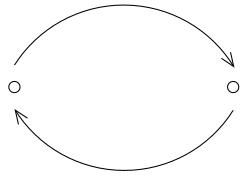
\includegraphics[width=0.25\textwidth]{sigma_i_configuration.png}
    \label{fig:sigma_i_configuration-png}
\end{figure}


\subsection{Mapping Class Group of a punctured disk}

Let $D_n$ be a closed disk $D^2$ with $n$ marked points.
Then
\[
B_n \approx \Mod\left( D_n \right) =
\pi_0 \left( \Homeo^{+} \left( D_n, \partial D_n \right)  \right).
\] 

To see this, let $\varphi$ be a representative
of some element in $\Mod \left( D_n \right) $ which
leaves the set of marked points invariant under
$\varphi$ - i.e., if $\left\{ x_0, \ldots,x_n \right\} 
\subset D_n$ are the $n$ marked points, then
$\varphi \left( \left\{ x_0, \ldots,x_n \right\}  \right) 
= \left\{ x_0, \ldots, x_n \right\} $. Note that we
do not regard these marked points as punctures because
we will not want to consider isotopies which "move" these
marked points around which is not allowed when the marked points
represent punctures.
We see that
$\varphi $ is simply a homeomorphism of $D^2$ fixing
$\partial D^2$ pointwise, so by the Alexander
lemma, $\varphi $ is isotopic to the identity. Now, throughout
such an isotopy, the marked points must again be send to
themselves, albeit they might move around through
in the interior of $D^2 $ (which we identify with
$\mathbb{C}$ ) throughout the isotopy. Thus
this isotopy produces a loop of these marked points,
i.e., it produces a loop in $C \left( \mathbb{C},n \right) $.
So we have produced a braid.

\begin{question}\label{question-1}
    Does this association give a well-defined homomorphism
    $B_n \to \Mod(D_n) $ and would this be an isomorphism?
\end{question}

The answer is yes, and since $\sigma_i$ generate
$B_n$, the images generate $\Mod(D_n)$. Now, the
image of $\sigma_i$ will be the
homotopy class of a homeomorphism
of $D_n$ that has support a twice-punctured disk and is
described on this support by figure \ref{fig:half-twist-png}.

\begin{figure}[htpb]
    \centering
    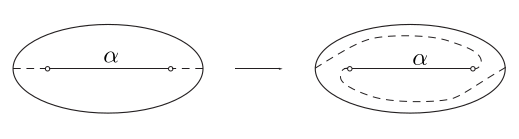
\includegraphics[width=0.5\textwidth]{half-twist.png}
    \caption{A half-twist}
    \label{fig:half-twist-png}
\end{figure}

We denote such a half-twist as $H_{\alpha}$, and we
can think of $\alpha$ as either a simple closed
curve with two punctures in its interior or a simple
proper arc connecting two punctures.


\subsection{The Birman Exact Sequence}

Let $S$ be any surface, possibly with punctures (but no 
marked points) and let
$\left( S, x \right) $ denote the surface obtained
from $S$ by marking a point $x$ in the
interior of $S$. There is a natural
homomorphism
\[
\Forget \colon \Mod \left( S, x \right) \to \Mod(S)
\] 
called the forgetful map which is realized by forgetting
that the point $x$ is marked. This map is
surjective as any homeomorphism of $S$ can
be modified by isotopy to fix $x$ (why?). The
group $\Mod(S,x)$ is isomorphic to the
subgroup $G$ of $\Mod \left( S - x \right) $ 
consisting of homeomorphisms preserving the
puncture coming from $x$.

The forgetful map can then be interpreted
as the map $G \to \Mod(S)$ obtained by "filling in" the
puncture $x$. I.e., $\Forget$ is the map
induced by the inclusion
 $S -x \hookrightarrow S$.



 

 \subsubsection{Analyzing the kernel of $\Forget$}

 Let $f \in \Mod(S,x)$ be an element of the kernel
 of $\Forget$ and let  $\varphi $ be a homeomorphism
 representing $f$. We can think of
 $\varphi $ as a homeomorphism $\overline{\varphi}$ of
 $S$.

 Since $\Forget (f) = 1$, there is an isotopy
 from $\overline{\varphi }$ to $\mathbbm{1}_S$. During
 this isotopy, the image of the point $x$ traces out a
 loop $\alpha$ in $S$ based at $x$. Now
 we will introduce the $\Push$ map:
 given a loop $\alpha$ in $S$ based at $x$, we can
 consider $\alpha \colon \left[ 0,1 \right] \to S$ as
 an isotopy $h \colon \left\{ x \right\} \times I
 \to S$ with $h(x,0) = h(x,1) = x$ and extend this
 to the whole surface using \ref{Hirsch-isotopy-extension} (here,
 $V = \left\{ x \right\} $ ), denote this by
 $h \colon S \times I \to S$ also. Let
 $\varphi (x) = h(x,1) $ be the homeomorphism
 of $S$ obtained at the end of the isotopy. Taking its
 isotopy class in $\Mod \left( S,x \right) $, we get
 $\left[ \varphi  \right] = : 
 \Push(\alpha) \in \Mod\left( S,x \right) $.
 Think of $\Push(\alpha)$ as placing your finger on
 $x$ and pushing $x$ along $\alpha$, draggin the
 rest of the surface along as you go (indeed, locally,
 this is what must happen).

 The question of whether this mapping class
 is independent of the choice of isotopy extension
 as well as the choice of $\alpha$ within its homotopy class.
 I.e., whether $\Push$ defines a 
 well-defined map
 \[
 \Push \colon \pi_1 \left( S,x \right) 
 \to \Mod \left( S,x \right) .
 \] 
 For that, we show look at the
 Birman exact sequence.






 \begin{theorem}[Birman exact sequence]
     Let $S$ be a surface with $\chi (S) < 0$, possibily
     with punctures and/or boundary. Let
     $\left( S, x \right) $ be the surface
     obtained from $S$ by marking a point $x$ in
     the interior of $S$. Then the following
     sequence is exact:
     \[
         1 \to \pi_1 \left( S, x \right) \stackrel{\Push}{\to }
         \Mod \left( S, x \right) 
         \stackrel{\Forget}{\to } \Mod(S) \to 1.
     \] 
 \end{theorem}


 \begin{lemma}[]
     $\Push \colon \pi_1 \left( S,x \right) 
     \to \Mod (S,x)$ is injective when
     $\chi (S) <0$.
 \end{lemma}

 \begin{proof}
     Let $\varphi $ represent 
     $\Push \left( \alpha \right) \in 
     \Mod \left( S,x \right) $. Then
     $\varphi $ is a map
     $\left( S,x \right) \to \left( S,x \right) $, so
     in particular, we have an induced homomorphism
     $\varphi_* \colon \pi_1 \left( S,x \right) 
     \to \pi_1 \left( S,x \right) $.
     This homomorphism is the inner automorphism
     $I_{\alpha} (\gamma) = \alpha \gamma \alpha^{-1}$ (why?).
     Now, for $\chi (X) < 0$, the center of $\pi_1 (S)$ is
     trivial, so $I_{\alpha}$ is nontrivial whenever
     $\alpha \neq c_{x}$. If $\varphi $ had been
     homotopic to the identity, their
     induced homomorphisms would be equal, so we conclude
     that $\Push \left( \alpha \right) $ is nontrivial whenever
     $\alpha$ is nontrivial.
 \end{proof}

 \subsubsection{Push maps along loops in terms of Dehn twists}

 Let $\alpha \in \pi_1 \left( S,x \right) $ be simple.
 Let $S^{1} \times \left[ 0,2 \right] $ be an annulus
 about $\alpha$ with $S^{1} \times \left\{ 1 \right\} $ 
 identified with $\alpha$ with
 $(0,1)$ identified with the marked point
 $x$. We orient 
 $S^{1} \times \left[ 0,2 \right] $ with the
 standard orientations on
 $S^{1}$ and $\left[ 0,2 \right] $. 

 Let $F \colon A \times I \to A$ be the
 isotopy given by
 \[
 F \left( \left( \theta,r \right) ,t \right) 
 = 
 \begin{cases}
     \left( \theta + 2\pi r t, r \right) ,& 0 \le r \le 1\\
     \left( \theta + 2 \pi (2-r)t,r \right) ,& 1 \le r \le 2.
 \end{cases}
 \]
 By \ref{Hirsch-isotopy-extension}, we can extend
 $F$ to an ambient isotopy of $S$. Restricting
 $F$ to $\left\{ x \right\} \times \left[ 0,1 \right] $, we
 get
 \[
 F\left( (0,1),t \right) = \left( 2 \pi t,1 \right),
 \] 
 so $F$ pushes $x$ around the core of the annulus.
 Now, the homeomorphism (representing $\Push\left( \alpha \right) $ )
 $\varphi $ of $\left( S,x \right) $ given by
 $F\left( (\theta, r),1 \right) $ is a product
 of two Dehn twists,  $T_a T_{b}^{-1}$ where
 $a$ is the closed curve identified with
 $S^{1} \times \left\{ 0 \right\} $ and
 $b$ is the closed curve identified with
 $S^{1} \times \left\{ 2 \right\} $.

 \begin{figure}[htpb]
     \centering
     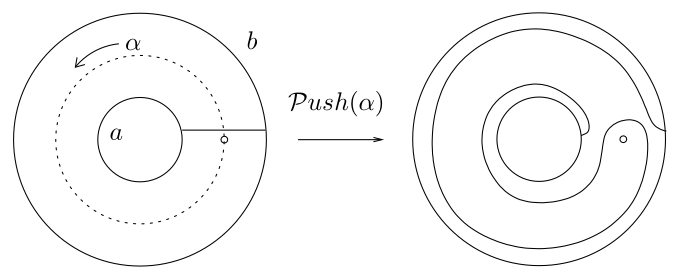
\includegraphics[width=0.7\textwidth]{push-point-map.png}
     \label{fig:push-point-map-png}
 \end{figure}

 \begin{remark}[Naturality]
     For any $h \in \Mod (S,x)$ and any
     $\alpha \in \pi_1 \left( S,x \right) $, we have
     \[
     \Push \left( h_* \left( \alpha \right)  \right) 
     = h\Push \left( \alpha \right) h^{-1}.
     \] 
 \end{remark}



 \begin{proof}
     Write a proof of the Birman exact sequence.
 \end{proof}

 \subsection{Generalized Birman Exact Sequence}

 We now return to Question \ref{question-1}.
 We wish to show that $\pi_1 \left( C
 \left( \mathbb{C},n \right) \right) \approx
 \Mod \left( D_n \right) $. 

 \begin{definition}[$n$-stranded surface braid group of
     $S$]
     For an arbitrary surface $S$, we
     call $\pi_1 \left( C \left( S,n \right)  \right) $ 
     the $n$-stranded surface braid group of $S$.
 \end{definition}

 Let $S$ be a compact finite-type surface without marked
 points. Let $\left( S, \left\{ x_1, \ldots, x_n \right\}  \right) $ 
 denote $S$ with $n$ marked points $x_1, \ldots, x_n$ in
 the interior. Equivalently to the construction
 in the proof of the Birman exact sequence,
 there is a fiber bundle
 \[
 \Homeo^{+} \left( \left( S,
 \left\{ x_1, \ldots, x_n \right\} \right), \partial S  \right) 
 \to \Homeo^{+} \left( S, \partial S \right) 
 \to C \left( S^{\circ},n \right) 
 \]
 where $S^{\circ}$ is the interior of
 $S$ and $\Homeo^{+} \left( \left( S,
 \left\{ x_1,\ldots,x_n \right\} \right) ,\partial S \right) $ 
 is the group of orientation-preserving homeomorphisms
 of $S$ that preserve the set
 $\left\{ x_1,\ldots,x_n \right\} $ (allowing permutations,
 however) and fix the boundary of $S$ pointwise.

 \begin{theorem}[Birman exact sequence generalized]
     Let $S$ be a surface without marked points
     and with $\pi_1 \left( \Homeo^{+} \left( 
     S, \partial S\right)  \right) = 1$. The following
     sequence is exact:
     \[
     1 \to \pi_1 \left( C \left( S,n \right)  \right) 
     \stackrel{\Push}{\to } \Mod \left( S,
     \left\{ x_1, \ldots, x_n \right\} \right) 
     \stackrel{\Forget}{\to } \Mod (S) \to 1.
     \] 
 \end{theorem}


 \begin{corollary}
     When $S = D^2$, this gives the exact sequence
     \[
         1 \to
         \underbrace{\pi_1 \left( C \left( D^2,n \right)\right)}_{B_n}
     \to \Mod \left( D_n \right) \to 
     \underbrace{\Mod \left( D^2 \right)}_{1} \to 1.
     \] 
     Hence $B_n \approx \Mod \left( D_n \right) $.
 \end{corollary}

 \subsection{Algebraic Structure of the Braid Group}

 \newpage

 \subsection{The pure braid group}

 Recall that by definition of a braid group, we
 are given a collection of $n$ points
 $p_1, \ldots, p_n$, $n$ paths
 $f_i \colon I \to \mathbb{C} \times I$ and
 a permutation $\overline{f} \in \Sigma_n$ such that
 $f_i(0) = p_i$
 and $f_i(1) = p_{\overline{f}(i)}$.
 We can thus define a homomorphism
 $B_n \to \Sigma_n$ by sending
 $f \mapsto \overline{f}$.
 \begin{definition}[]
     We define the \textit{pure braid group} $PB_n$ as
     the kernel of the homomorphism
     $B_n \to \Sigma_n$ given by $f \mapsto \overline{f}$.
 \end{definition}
 We obtain the short exact sequence
 \[
 1 \to PB_n \to B_n \to \Sigma_n \to 1.
 \] 
 So a pure braid is a braid where each strand begins
 and ends at the same point of $\mathbb{C}$.

 \begin{exercise}[]
     Show that
     \[
     PB_n \approx \pi_1 \left( C^{ord } 
     \left( \mathbb{C},n \right) \right) \approx
     \PMod (D_n)
     \] 
 \end{exercise}


 \newpage

 \subsection{Braid group and symmetric mapping class groups}

 Let $S_{g}^{1}$ be a surface of genus $g$ with
 one boundary component. Define a
 homomorphism $\psi \colon B_n \to 
 \Mod \left( S_g^{1} \right) $ for
 $n \le 2g+1$ as follows.
 Choose a chain of simple closed curves
 $\left\{ \alpha_i \right\} $ in
 $S_{g}^{1}$, that is, a collection of
 simple closed curves satisfying
 $i \left( \alpha_i, \alpha_{i+1} \right) =1$ for
 all $i$ and $i \left( \alpha_i, \alpha_j \right) =0$ otherwise.
 We then define $\psi $ via
 $\psi \left( \sigma_i \right) =
 T_{\alpha_i}$.
 This is well defined if and only if
 $T$ respects all the relations in
 $B_n$. Now, if $\sigma_i$ and
 $\sigma_j$ are given with 
 $\left| i-j \right| \ge 2$, then
 $\sigma_i \sigma_j = \sigma_j \sigma_i$ and
 indeed also
 $i \left( \alpha_i, \alpha_j \right) =0$ so
 by the disjointness relation for
 Dehn twists (fact 3.9), we get
 that $T$ respects this commutativity.

 Similarly, we have that
 $\sigma_i \sigma_{i+1} \sigma_i$, for all $i$,
 is mapped to 
 $T_{\alpha_i} T_{\alpha_{i+1}} T_{\alpha_i}$ which, by the
 braid relation on Dehn twists and the
 assumption that
 $i\left( \alpha_i, \alpha_{i+1} \right) =1$ for all $i$,
 is equivalent to
 $T_{\alpha_{i+1}} T_{\alpha_i}T_{\alpha_{i+1}}$, so
 the braid relation in $B_n$ is respected
 under $\psi $.

 \begin{question}
     Can we say whether $\psi $ is injective?
 \end{question}

 \subsection{The Birman-Hilden Theorem}
Let $\iota$ be the order  $2$ element of
$\Homeo^{+} \left( S_g^{1} \right) $ as
shown in figure \ref{fig:birman-hilden-double-cover-png}
and let $\SHomeo^{+} \left( S_g^{1} \right) $ be
the centralizer in
$\Homeo^{+}\left( S_g^{1}, \partial S_g^{1} \right) $ of
$\iota$:
\[
\SHomeo^{+} \left( S_g^{1} \right) 
= C_{\Homeo^{+} \left( S_g^{1}, \partial
S_g^{1} \right) }\left( \iota \right) .
\] 

 \begin{figure}[H]
     \centering
     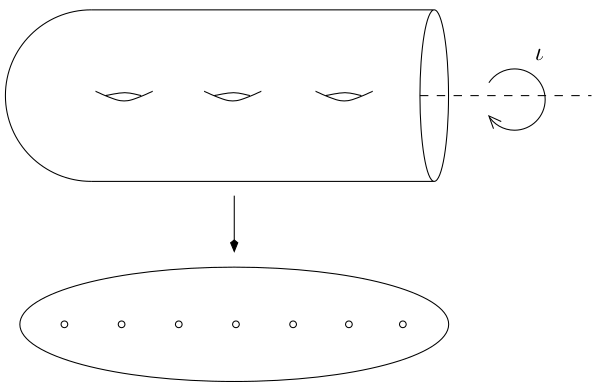
\includegraphics[width=0.6\textwidth]{birman-hilden-double-cover.png}
     \caption{The Birman-Hilden double cover}
     \label{fig:birman-hilden-double-cover-png}
 \end{figure}

 \begin{definition}[]
 The group $\SHomeo^{+} \left( S_g^{1} \right) $ is
 called the group of orientation-preserving
 symmetric homeomorphisms of $S_g^{1}$. 
 The symmetric mapping class group is the group
 \[
 \SMod (S_g^{1}) = 
 \SHomeo^{+} \left( S_g^{1} \right) / \text{isotopy},
 \] 
 i.e, the subgroup of $\Mod \left( S_g^{1} \right) $ that
 is the image of $\SHomeo^{+} \left( S_g^{1} \right) $.
 \end{definition}

 The homeomorphism $\iota$ has
  $2g+1$ fixed points in
   $S_g^{1}$. The quotient of
   $S_g^{1}$ by $\left<\iota \right>$ is
   a topological disk
   $D_{2g+1}$ with $2g+1$ cone points of order
   $2$, with each cone point coming from a fixed point of $\iota$.
   Since the elements of  $\SHomeo^{+} \left( S_g^{1} \right) $ 
   commute with $\iota$, they descend to homeomorphisms
   of the quotient disk, and by the commutativity, they
   must preserve the set of  $2g+1$ fixed points of $\iota$,
   and so there is a homomorphism
    \[
   \SHomeo^{+} \left( S_g^{1} \right) 
   \to \Homeo^{+} \left( D_{2g+1}, \partial D_{2g+1} \right) 
   \] 
   by sending
   $\varphi $ to
   $\pi \circ \varphi $ where
   $\pi \colon S_g^{1} \to 
   D_{2g+1}$ is the quotient map. If
   $\varphi  \mapsto \pi \circ \varphi  = \mathbbm{1}_{
   D_{2g+1}}$, then $\varphi  
   \in \left<\iota \right>$, and since $\iota 
   \not\in \SHomeo^{+} \left( S_g^{1} \right) $, we have
   $\varphi  = 1$.
   


   \begin{question}
       Why does any
   element of $\Homeo^{+} \left( D_{2g+1} \right) $ 
   lift to $\SHomeo^{+} \left( S_g^{1} \right) $?
   \end{question} 

   \begin{definition}[]
       We say two homeomorphisms
       $\varphi , \psi \in \SHomeo^{+}\left( S_g^{1} \right) $ 
       are symmetrically isotopic whenever
       $\left[ \varphi  \right] =
       \left[ \psi \right] $ in
       $\pi_0 \left( \SHomeo^{+}\left( S_g^{1} \right)  \right) $.
       Note that here,
       $\SHomeo^{+} \left( S_g^{1} \right) $ inherits
       the subspace topology from
       $\Homeo^{+} \left( S_{g}^{1} \right) $ 
       (actually, is this true?...)
   \end{definition}

   If we have this, we get an isomorphism of the
   two, so
   \begin{align*}
       \SHomeo^{+} \left( S_g^{1} \right) /
       \text{symmetric isotopy}
       &= \pi_0 \left( \SHomeo^{+}(S_g^{1}) \right) \\
       &\approx \pi_0 \left( \Homeo^{+} \left( 
       D_{2g+1}, \partial D_{2g+1} \right)  \right) \\
       &= \Mod \left( D_{2g+1} \right) \\
       &\approx B_{2g+1}.
   \end{align*}
   
   We want to show that
   if two symmetric homeomorphisms of $S_{g}^{1}$ are
   isotopic, then they must be symmetrically isotopic.
 

   \subsection{The Birman-Hilden Theorem}

   \begin{theorem}[Birman-Hilden]
       $\SMod \left( S_g^{1} \right) \approx
       B_{2g+1}$.
   \end{theorem}


   \begin{example}[]
       Taking $g=1$, we will find
       $\Mod \left( S_g^{1} \right) $.
       Note that by corollary
       \ref{hyperelliptic-involution-in-center},
       $\iota \in C\left( 
       \Homeo^{+}\left( S_g^{1} \right)  \right)  $, so
       $\Mod \left( S_1^{1} \right) =
       \SMod\left( S_g^{1} \right) $, and now it is
       easy to see that
       \[
       \Mod \left( S_1^{1} \right) = \SMod \left( S_g^{1} \right) 
       \approx B_{3} \approx \Mod \left( D_3 \right) 
       \] 
   \end{example}

   \begin{remark}[]
       The Birman-Hilden theorem also holds for
       surfaces with two symmetric boundary
       components that are interchanged by
       $\iota$, see figure
       \ref{fig:-Birman-Hilden-two-symmetric-boundary-components-png}.
        \begin{figure}[htpb]
           \centering
           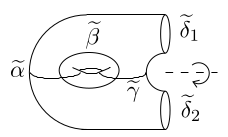
\includegraphics[width=0.3\textwidth]{
           Birman-Hilden-two-symmetric-boundary-components.png}
           \caption{Symmetric boundary components
           interchanged by $\iota$.}
           \label{fig:-Birman-Hilden-two-symmetric-boundary-components-png}
       \end{figure}
       Hence
       \[
       \SMod \left( S_g^{2} \right) 
       \approx B_{2g+2}.
       \] 
   \end{remark}





   \subsection{Proof of the Birman-Hilden Theorem}

   \begin{definition}[]
       A closed curve $\alpha$ in $S_g$ is symmetric
       if $\iota \left( \alpha \right) = \alpha$ as sets.
   \end{definition}

   \begin{lemma}[]
       Let $g \ge 2$ and let $\alpha$ and $\beta$ be
       two symmetric nonseparating simple closed
       curves in $S_g$. If $\alpha$ and $\beta$ are isotopic,
       then they are symmetrically isotopic.
   \end{lemma}

   \begin{proof}
       Let $\overline{\alpha}$ and $\overline{\beta}$ 
       denote the images of $\alpha$ and $\beta$ 
       in $S_{0,2g+2}\approx S_g / \left<\iota \right>$.
       Now,
       $ \overline{\alpha}$ and $ \overline{\beta}$
       must be simple proper arcs in $S_{0,2g+2}$ (look
       at it geometrically - in particular, remember $\alpha$ and
       $\beta$ are symmetric).

       Let's look at an example to get a picture. If
       $\alpha$ and $\beta$ are symmetric choices of the
       usual generating loops in the homology of a torus, these
       will correspond to one loop being the
       "innermost" meridian loop while we choose the
       other loop to be a longitudinal loop
       whose plan of existence is
       normal to the axis of rotation. See
       figure~\ref{fig:homology-basis-of-torus-and-double-torus-png}.

       \begin{figure}[htpb]
           \centering
           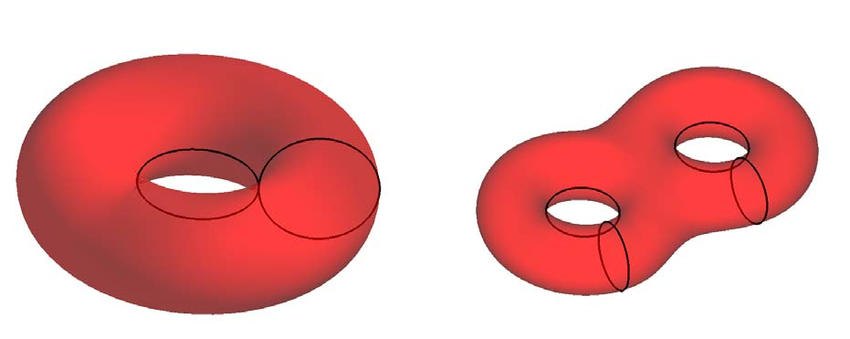
\includegraphics[width=0.8\textwidth]{homology-basis-of-torus-and-double-torus.png}
           \caption{Basis for homologies of torus and
           double torus}
           \label{fig:homology-basis-of-torus-and-double-torus-png}
       \end{figure}
       Imagine in this figure now we cut the surface into a "lower"
       and "upper" half. Looking at the resulting paths of
       our loops, we indeed get arcs for the longitudinal loops
       and loop on the boundary for the meridian loops.




       
       Now, an isotopy between
       these arcs will lift to a symmetric isotopy
       between $\alpha$ and $\beta$.


       I.e., if
       $H$ is an isotopy between $\alpha$ and $\beta$, then
       there exist an induced map $\tilde{H}$ such that
       \begin{equation*}
       \begin{tikzcd}
           & S_g \ar[d] \\
           I^2 \ar[ru, "\tilde{H}"] \ar[r, "H"'] &
           S_g / \left<\iota \right>
       \end{tikzcd}
       \end{equation*}
       commutes since $I^2$ is simply connected,
       path-connected and locally path-connected
       \cite[Cor~4.2]{Bredon}.
       
       We can modify $\alpha$ by a symmetric
       isotopy so that it is transverse to $\beta$.
       We claim that $\alpha$ cannot be
       disjoint from $\beta$. Indeed,
       for then $\overline{\alpha}$ and $\overline{\beta}$ 
       are disjoint including endpoints. But
       such arcs cannot correspond
       to isotopic curves in $S_g$: we can choose
       an arc $\overline{\gamma}$ that passes through
        an odd number of endpoints of
        $\overline{\alpha}$ and
        an even number of endpoints of $\overline{\beta}$.
        This will then lift to a loop
        $\gamma$ in $S_g$ with
        $i \left( \alpha, \gamma \right) $ odd
        and $i \left( \beta, \gamma \right) $ even, contradicting
        $\alpha$ isotopic to $\beta$.

        Now, since $\alpha$ is isotopic to $\beta$ and
        $\alpha \cap \beta \neq \varnothing$, the bigon
        criterion gives that
        $\alpha$ and $\beta$ form a bigon $B$. Assume
        $B$ is the innermost bigon. As
        $\alpha$ and $\beta$ are fixed (they are symmetric) by
        $\iota$, we have that $\iota (B)$ is another
        innermost bigon in the graph
        $\alpha \cup \beta$.

        But $\iota$ reverses the orientation of non-separating
        closed curves (while preserving orientations
        of separating closed curves), so
        since the bigon $B$ lies to one side of $\alpha$,
        $\iota(B)$ must lie on the other side of $\alpha$.\\
        \linebreak
        It follows that the image of 
        $B$ in $S_{0,2g+2}$ is an innermost bigon $\overline{B}$ 
        between $\overline{\alpha}$ and $\overline{\beta}$ (why?).
        Furthermore, since $\iota (B) \neq B$, there are
        no fixed points of $\iota$ in $B$ and hence
        no marked points of
        $S_{0,2g+2}$ in $\overline{B}$.

        Now, considering the boundary of the bigon $\overline{B}$,
        it can have zero, one or two of its vertices on
        marked points of $S_{0,2g+2}$. In the first two cases,
        we can modify $\overline{\alpha}$ by isotopy
        in order to remove the bigon (why?), reducing the intersection
        number of $\overline{\alpha}$ and $\overline{\beta}$.
        In the last case, since $\overline{B}$ is innermost,
        we see that $\overline{\alpha} \cup 
        \overline{\beta}$ is a simple loop bounding
        a disk (why?), and we can push $\overline{\alpha}$ onto
        $\overline{\beta}$. Removing bigons inductively,
        we see that $\overline{\alpha}$ is isotopic
        to $\overline{\beta}$, and this isotopy lifts to a
        symmetric isotopy between $\alpha$ and $\beta$.

   \end{proof}

   \begin{proposition}[]
       Let $g \ge 2$ and let $\varphi , \psi \in 
       \SHomeo^{+} (S_g)$. If $\varphi $ and $\psi$ are
       isotopic, then they are symmetrically isotopic.
   \end{proposition}

   \begin{proof}[Proof of the Birman-Hilden theorem]
       We have a commutative diagram
       \begin{equation*}
       \begin{tikzcd}
           \SHomeo^{+} (S_g) \ar[r, twoheadrightarrow] & 
           \Homeo^{+}\left( S_{0,2g+2}, \partial
           S_{0,2g+2}\right) 
           \ar[rr] \ar[dr] & & \Mod \left( S_{0,2g+2} \right) \\
                           & & \SMod(S_g)  \ar[ru] &
       \end{tikzcd}
       \end{equation*}

       We wish to find the kernel of
       the map $\SMod (S_g) \to \Mod \left( S_{0,2g+2} \right) $.
       Suppose $f \in \SMod(S_g)$ is mapped
       to $0$. Since the composition
       $\SHomeo^{+}(S_g) \to \Homeo^{+} \left( S_{0,2g+2} \right) 
       \to \Mod \left( S_{0,2g+2} \right) $ is a surjective
       homomorphism, we can choose a representative
       $\varphi  \in \SHomeo^{+} \left( S_g \right) $.
       Let $\overline{\varphi  }$ be the image
       in $\Homeo^{+} \left( S_{0,2g+2} \right) $.
       Then $\overline{\varphi }$ is isotopic to
       the identity, say $H \colon I^2 \to 
       \Homeo^{+} \left( S_{0,2g+2} \right) $. Then
       this lifts to a symmetric isotopy
       $\tilde{H} \colon I^2 \to \SHomeo^{+} \left( S_g \right) $ 
       making the following diagram commute

       \begin{equation*}
       \begin{tikzcd}
           & I^2 \ar[dl, "\tilde{H}"'] \ar[dr, "H"] & & &\\
           \SHomeo^{+} (S_g) \ar[rr, twoheadrightarrow] & &
           \Homeo^{+}\left( S_{0,2g+2}, \partial
           S_{0,2g+2}\right) 
           \ar[rr] \ar[dr] & & \Mod \left( S_{0,2g+2} \right) \\
                           &  & & \SMod(S_g)  \ar[ru] &
       \end{tikzcd}
       \end{equation*}
       Now, $\tilde{H}$ is an isotopy of $\varphi $ to
       either the identity or $\iota$, so
       \[
       \SMod \left( S_g \right) / \left<\left[ \iota \right]  \right>
       \approx \Mod \left( S_{0,2g+2} \right) .
       \] 
       
   \end{proof}


   \begin{remark}[]
       We can generalize the proof of the Birman-Hilden
       theorem a bit to the case of $S_g^{1}$ quite simply:
       the quotient of $S_g^{1}$ by the hyperelliptic
       involution $\iota \colon S_g^{1}\to 
       S_g^{1}$ is a disk with $2g+1$ marked points.
       Since  $\iota \colon S_g^{1} \to 
       S_g^{1}$ is not an element of
       $\Homeo^{+}\left( S_g^{1}, \partial
       S_g^{1}\right) $, it does not represent an
       element of $\SMod(S_g^{1})$, and so we 
       get 
       \[ \SMod \left( S_g^{1} \right) 
       \approx \Mod \left( D_{2g+1} \right) 
   \approx B_{2g+1}.\]
   \end{remark}




   \newpage


   \section{Braided monoidal categories}


   \subsection{Monoidal categories}

   We first introduce the notion of a monoidal category.

   \begin{definition}[Monoidal category]
       A monoidal category is a tuple
       $V = \left( V, \otimes, I, a, l ,r \right) $ consisting
       of a category $V$, a functor
       $\otimes \colon V \times V \to V$ called the
       tensor product, and object $I \in V$ called the
       unit, and natural isomorphisms
       \begin{align*}
           a &\colon \left( - \otimes - \right) \otimes -
           \stackrel{\sim}{\implies} - \otimes \left( - 
           \otimes - \right)\\
           l &\colon I \otimes - \stackrel{\sim}{\implies} -\\
           r &\colon - \otimes I \stackrel{\sim}{\implies} -
       \end{align*}
       called the associativity, left unit and right unit
       constraints, respectively. 
       Additionally, we require that for all
       objects $A,B,C,D \in V$, the following two diagrams
       commute:\\[2 ex]

       \adjustbox{scale=0.9,center}{
           \begin{tikzcd}
	&& {\left( A \otimes B  \right) \otimes \left(         C \otimes D \right)} \\
	{\left( \left( A \otimes B \right) \otimes C \right) \otimes D} &&&& {A \otimes \left( B   \otimes \left( C \otimes D \right) \right)} \\
	& {\left( A \otimes                                 \left( B \otimes C \right) \right)         \otimes D} && {A \otimes \left( \left( B \otimes C \right)         \otimes D \right)}
	\arrow["a", from=1-3, to=2-5]
	\arrow["a", from=2-1, to=1-3]
	\arrow["{a \otimes D}"', from=2-1, to=3-2]
	\arrow["a"', from=3-2, to=3-4]
	\arrow["{A \otimes a}"', from=3-4, to=2-5]
\end{tikzcd}
   }
   \\[1 ex]
   and
   \\[1 ex]

   \adjustbox{scale=0.9,center}{
   \begin{tikzcd}
	{(A \otimes I) \otimes B} && {A \otimes (I \otimes B)} \\
	& {A \otimes B}
	\arrow["a", from=1-1, to=1-3]
	\arrow["{r \otimes B}"', from=1-1, to=2-2]
	\arrow["{A \otimes l}", from=1-3, to=2-2]
\end{tikzcd}
}

The monoidal category is called strict when all the
natural isomorphisms are identity morphisms for all objects.
   \end{definition}

   \begin{definition}[Braiding]
       A braiding for a monoidal category $V$ consists
       for a natural family of isomorphisms
       \[
           c = c_{A,B} \colon A \otimes B \stackrel{\sim}{\to }
           B \otimes A
       \] 
       in $V$ such that the following diagrams commute\\[3 ex]


       \begin{tikzcd}
	& {(B \otimes A) \otimes C} & {B \otimes (A \otimes C)} \\
	{(A \otimes B) \otimes C} &&& {B \otimes (C \otimes A)} \\
	& {A \otimes (B \otimes C)} & {(B \otimes C) \otimes A}
	\arrow["a", from=1-2, to=1-3]
	\arrow["{B \otimes c}", from=1-3, to=2-4]
	\arrow["{c \otimes C}", from=2-1, to=1-2]
	\arrow["a"', from=2-1, to=3-2]
	\arrow["c"', from=3-2, to=3-3]
	\arrow["a"', from=3-3, to=2-4]
\end{tikzcd}
\\[1 ex]
and \\[1 ex]
\begin{tikzcd}
	& {A \otimes (C \otimes B)} & {(A \otimes C ) \otimes B} \\
	{A \otimes (B \otimes C)} &&& {(C \otimes A) \otimes B} \\
	& {(A \otimes B) \otimes C} & {C \otimes (A \otimes B)}
	\arrow["{a^{-1}}", from=1-2, to=1-3]
	\arrow["{c \otimes B}", from=1-3, to=2-4]
	\arrow["{A \otimes c}", from=2-1, to=1-2]
	\arrow["{a^{-1}}"', from=2-1, to=3-2]
	\arrow["c"', from=3-2, to=3-3]
	\arrow["{a^{-1}}"', from=3-3, to=2-4]
\end{tikzcd}
   \end{definition}


   \subsection{Braided monoidal category of decorated surfaces}

   \begin{definition}[Decorated surface]
       A decorated surface is a pair
       $(S,I)$ where $S$ is a compact connected
       surface with at least one boundary component
       and $I \colon \left[ -1,1 \right] 
       \hookrightarrow \partial S$ is a parametrised interval
       in its boundary.
   \end{definition}

   \begin{definition}[$\mathcal{M}_2$]
       Let $\mathcal{M}_2$ denote the groupoid where
       the objects are
       decorated surfaces and
       morphisms are isotopy classes of diffeomorphisms
       restricting to the identity on a neighborhood
       of $I$.
   \end{definition}

   We now construct a braided monoidal structure on
   $\mathcal{M}_2$ : given decorated surfaces
   $\left( S_1, I_1 \right) $ and
   $\left( S_2,I_2 \right) $, define
   $\left( S_1, I_1 \right) 
   \otimes \left( S_2, I_2 \right) 
   := \left( S_1 \# S_2, I_1 \# I_2 \right) $ to be
   the surface obtained by gluing
   $S_1$ and $S_2$ along the right half-interval
   $I_1^{+} \in \partial S_1$ and the
   left half-interval $I_2^{-} \in \partial S_2$, defining
   $I_1 \# I_2 = I_1^{-} \cup I_2^{+}$.

   \begin{figure}[htpb]
       \centering
       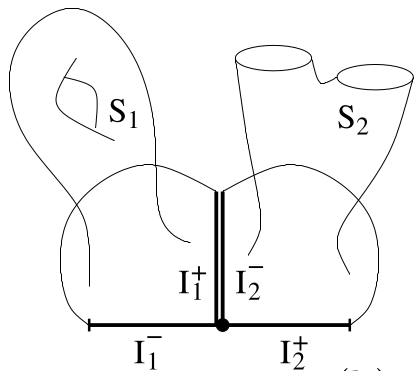
\includegraphics[width=0.35\textwidth]{connected-sum.png}
       \label{fig:connected-sum-png}
   \end{figure}

   Furthermore, we define the unit object to be
   $I := \left( D^2, I \right) $. 
   In this case, the monoidal structure is clearly strict. 

   We define a braiding $c$ on
   $\left( S_1 \# S_2, I_1 \# I_2 \right) $ 
   as the half-Dehn twist which satisfies that
   $c \colon \left( S_1 \# S_2, I_1 \# I_2 \right) 
   \stackrel{\sim}{\to } \left( S_2 \# S_1, I_2 \# I_1 \right)  $
   is a natural isomorphism because we
   it has the opposite half-Dehn twist as the inverse (why would
   this be natural?...)

   The B1 and B2 diagrams can be verified pictorially as follows:


   \begin{figure}[H]
    \centering
    \begin{minipage}[b]{0.5\textwidth}
        \centering
        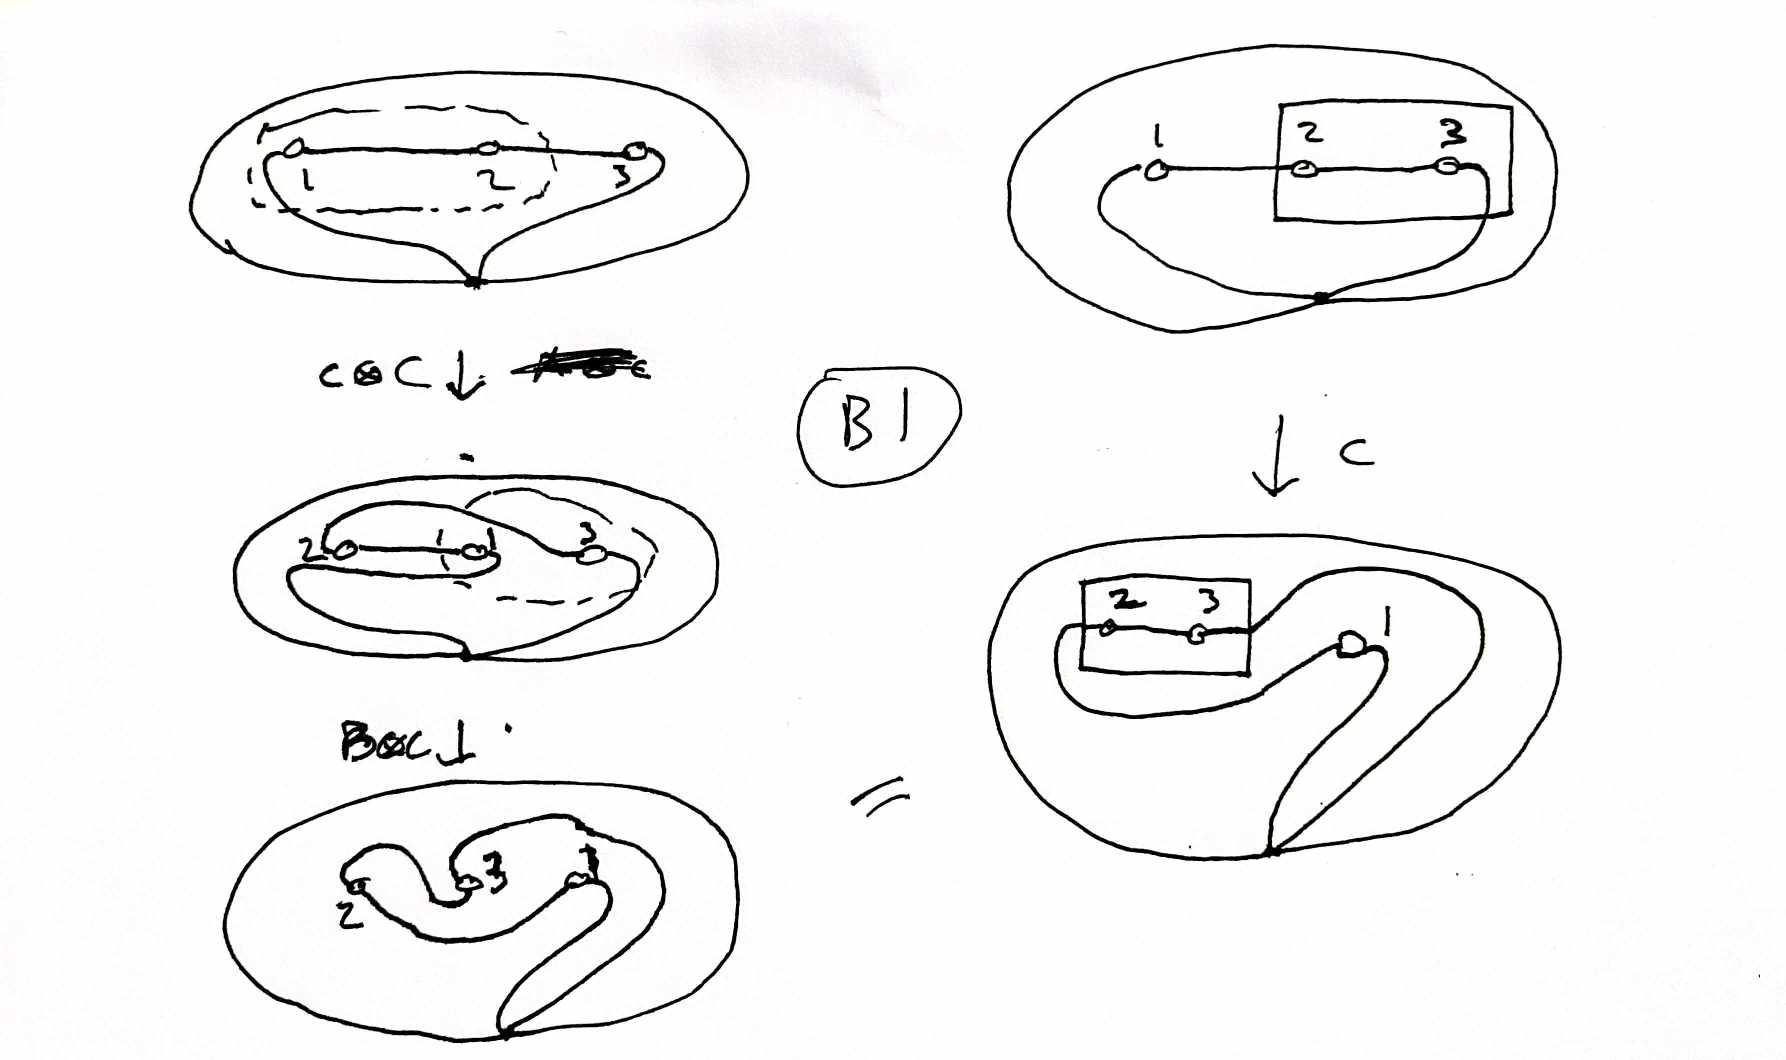
\includegraphics[width=1.1\textwidth]{B1.jpg} % first figure itself
    \end{minipage}\hfill
    \begin{minipage}[b]{0.5\textwidth}
        \centering
        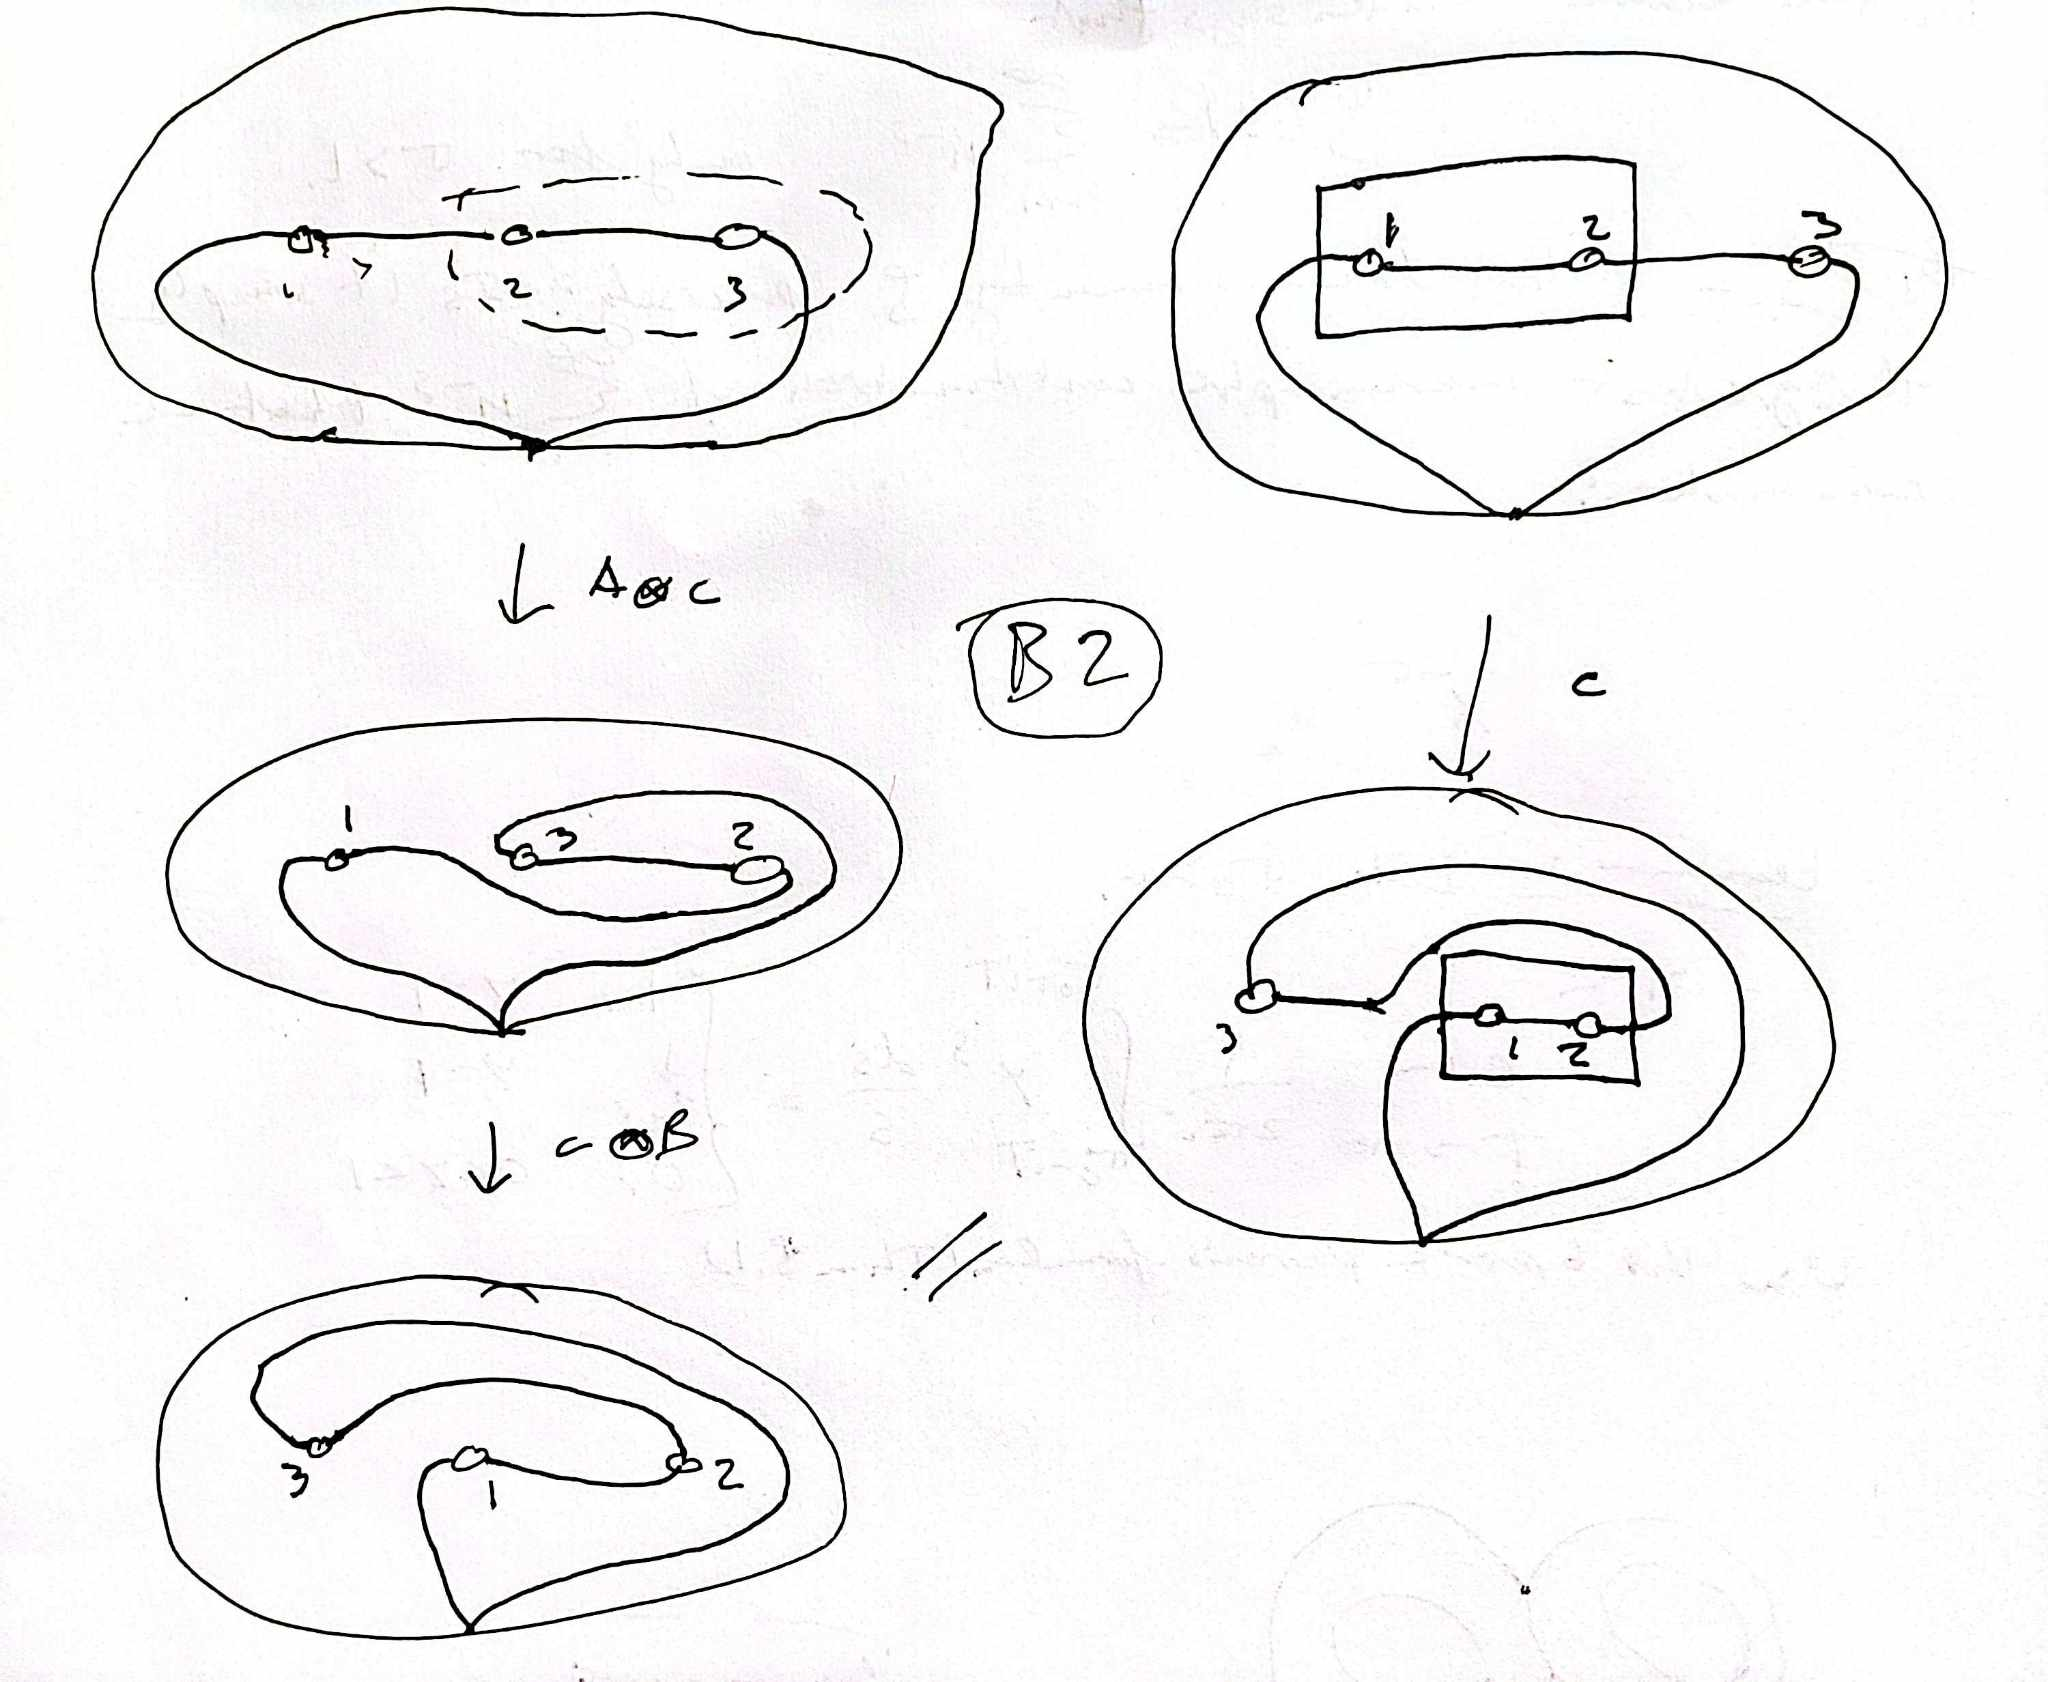
\includegraphics[width=0.9\textwidth]{B2.jpg} % second figure itself
    \end{minipage}
\end{figure}

\newpage 

\section{Geometric Representations of the Braid Group on
non-orientable surfaces}

A connected orientable (respectively nonorientable) surface
of genus $g$ with $b$ boundary components will
be denoted by $S_{g,b}$ (respectively $N_{g,b}$ ).

Now, recall that the Möbius band, which are also called
crosscaps), are the mapping cylinders on the map
$z \mapsto z^2$ (see figure~\ref{fig:mapping-cylinder-mobius})

\begin{figure}[htpb]
    \centering
    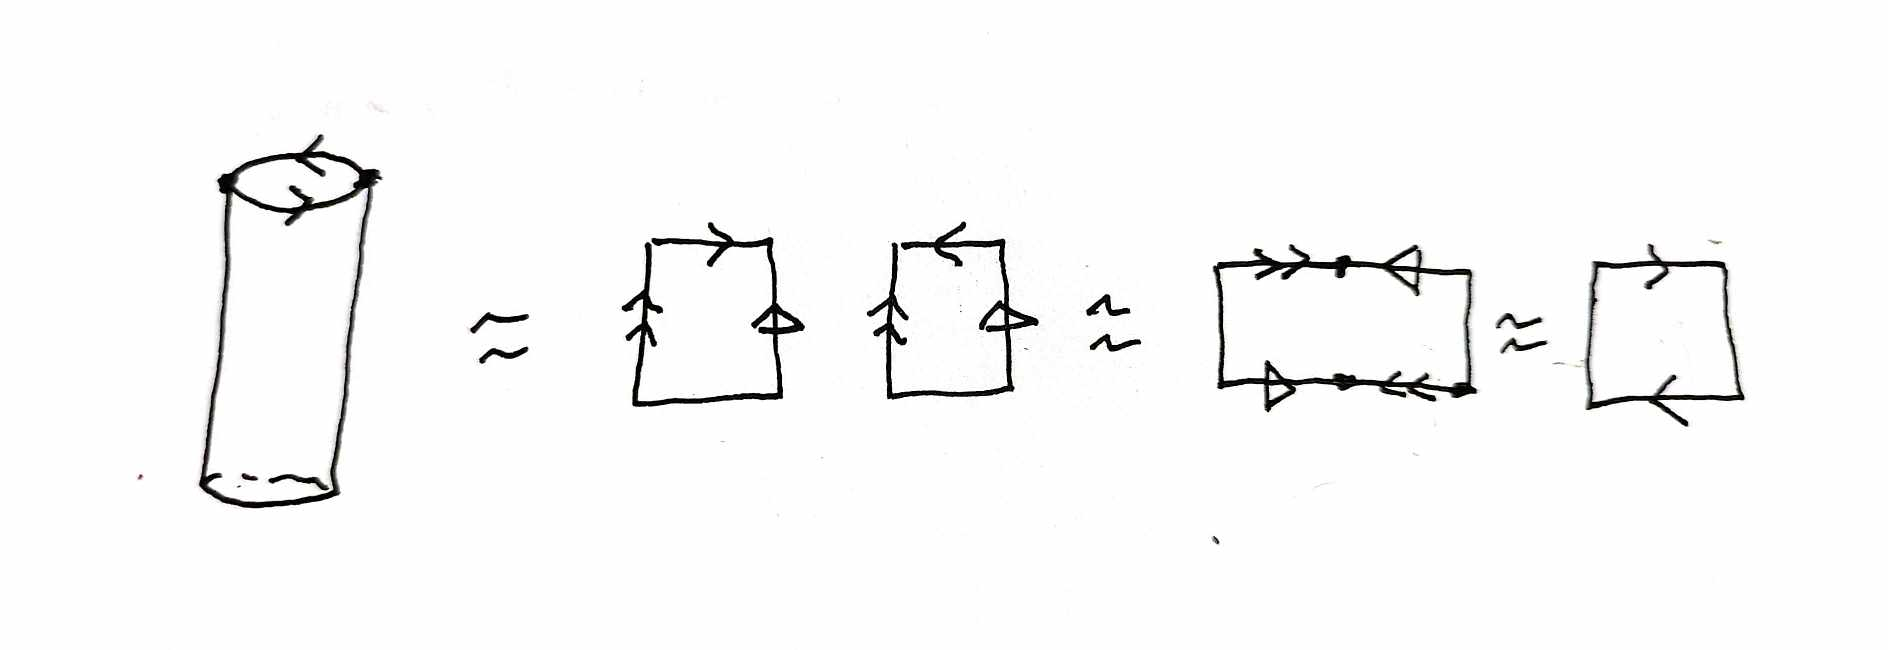
\includegraphics[width=0.7\textwidth]{mapping-cylinder-mobius.jpg}
    \label{fig:mapping-cylinder-mobius}
    \caption{Möbius band}
\end{figure}









\newpage

\section{Exercises}

\begin{problem}[]
    Give an example of a surface $S$ of finite type and
    self-diffeomorphism $\varphi $ of $S$ which is
    homotopic to $\id_S$ but not isotopic to $\id_S$.
\end{problem}

\begin{solution}
    Let $S$ be the closed
    unit disk $D^{1}$, and let $\varphi \colon D^{1} \to D^{1}$
    by the map $\left( x,y \right) \to (x,-y)$.
    This is a self-diffeomorphism which is homotopic to
    the identity map by
    $F \colon D^{1} \times I \to D^{1}$,
    $F(x,t) = \varphi(x) t + (1-t)x$. However,
    if there were an isotopy from $\id_S$ to 
    $\varphi$, then since this would have to be a topological embedding, it
    would have to map the boundary to the boundary at all
    times during the isotopy. But then restricting to the boundary,
    the isotopy would descend to an isotopy of
     $\id_{\partial D^{1}}$ to $\varphi|_{\partial D^{1}}$.
     However, these maps have degree $1$ and $-1$, respectively,
     and since degree is a homotopy invariant,
     we conclude that no such isotopy can exist.
\end{solution}




\newpage

\section{Glossary}

\begin{definition}[Equivariant maps]
    Suppose a group $G$ acts on spaces $X$ and $Y$, and let $f \colon X
    \to Y$ be a map. Then  $f$ is said to be equivariant if
    $f (g \cdot x) = g \cdot  f(x)$ for all $x \in X$ and all $g \in G$.
\end{definition}

\begin{definition}[Closed surface]
    A \textit{closed surface} is a surface that is compact
    and without boundary.
\end{definition}

\begin{definition}[Isotopy]
    A topological isotopy is a homotopy
    $F \colon X \times I \to Y$ such that for each $t_0 \in I$,
    $F(x,t_0) \colon X \to Y$ is a topological embedding (homeomorphism onto
    some subspace of $Y$ ).

    Two embeddings $f,g \colon X \to Y$ are said to be
    isotopic if there exists an isotopy $F \colon X \times I
    \to Y$ such that $F(x,0) = f(x)$ and $F(x,1) = g(x)$.
\end{definition}


\begin{definition}[Orientation]
    A closed $n$-manifold $M$ is called orientable
    if $H_n \left( M ; \mathbb{Z} \right) = \mathbb{Z}$.
    The choice of generator $\left[ M \right] $ in
    $\mathbb{Z}$ is called an orientation, and the generator
    is called the fundamental class of $M$. A manifold
    together with a choice of orientation is
    called oriented. A compact $n$-manifold $M$ with
    boundary is called orientable if
    $H_n \left( M, \partial M ; \mathbb{Z} \right) = \mathbb{Z}$.
    The choice of generator $\left[ M, \partial M \right] $ in
    $\mathbb{Z}$ is called an orientation, and
    $\left[ M, \partial M \right] $ is referred to as
    the fundamental class of $M$.

    A smooth manifold $M$ is orientable if and only if
    the restriction of its tangent bundle to every smooth
    curve is trivial.

    \begin{remark}[]
        This makes sense since T. Radó showed that every surface
        is triangulable and it is clear then that the $2$-cycles
        form a cyclic group. A choice of generator corresponds
        to choosing an orientation of each $2$-simplex in the
        triangulation (compatibly).
    \end{remark}
\end{definition}

\begin{definition}[Inner and outer automorphisms]
    Let $G$ be any group and $\gamma \in G$. A conjugate
    automorphism 
    \[
    I_{\gamma} \colon g \mapsto \gamma g \gamma^{-1}
    \] 
    is called an \textit{inner automorphism} of $G$.
    The group of inner automorphisms is denoted
    by $\text{Inn}(G)$. It is isomorphic to
    $G / Z(G)$, and is a normal subgroup of
    $\Aut(G)$. The quotient
    \[
    \text{Out}(G) := \Aut(G) / \text{Inn}(G)
    \] 
    is called the \textit{outer automorphism group} of
    $G$.
\end{definition}

\section{Appendix}

\subsection{Fiber Bundles}

\subsubsection{Bredon}

\begin{definition}[]
    Let $X, B$ and $F$ be Hausdorff spaces and
    $p \colon X \to B$ a map.
    Then $p$ is called a bundle projection with
    fiber $F$, if each point of
    $B$ has a neighborhood $U$ such that there
    is a homeomorphism $\varphi \colon U \times F \to 
    p^{-1}(U) $ such that $p \left( \varphi
    \left<b,y  \right>\right) = b$ for all $b \in U$ and
    $y \in F$. That is, on  $p^{-1}(U)$, $p$ corresponds
    to projection $U \times F \to U$. Such a map
    $\varphi $ is called a \textit{trivialization} of the
    bundle over $U$.
\end{definition}

\begin{definition}[]
    An action of a group $G$ on a space $X$ is
    said to be \textit{effective} if
    \[
        \left( \forall x \in X \colon
        gx = x \right) \implies g = e.
    \] 
\end{definition}

\begin{definition}[]
    Let $K$ be a topological group acting effectively on
    the Hausdorff space $F$ as a group of homeomorphisms.
    Let $X$ and $B$ be Hausdorff spaces. By a 
    \textit{fiber bundle} over the base space $B$ with
    total space $X$, fiber $F$, and
    structure group $K$, we mean a bundle projection
    $p \colon X \to B$ together with a collection
    $\Phi $ of trivializations $\varphi \colon
    U \times F \to p^{-1}(U)$, of $p$ over $U$, called
    \textit{charts} over $U$, such that
    \begin{enumerate}
        \item each point of $B$ has a neighborhood
            over which there is a chart in $\Phi $ ;
        \item if $\varphi \colon U \times F \to 
            p^{-1}(U)$ is in $\Phi $ and
            $V \subset U$ then the restriction
            of $\varphi $ to $V \times F$ is in $\Phi$;
        \item if $\varphi, \psi \in \Phi$ are
            charts over $U$, then there is a map
            $\theta \colon U \to K$ such that
            $\psi \left<u,y \right> = 
            \varphi \left<u , \theta(u) (y) \right>$ ;
        \item the set $\Phi $ is maximal among
            collections satisfying (1), (2) and (3).
    \end{enumerate}

    The bundle is called \textit{smooth} if all these spaces
    are manifolds and all maps involved are smooth.
\end{definition}




\begin{definition}[]
    A \textit{vector bundle} is a fiber bundle
    in which the fiber is a Euclidean space
    and the structure group is the general linear group
    if this Euclidean space or some subgroup of that
    group.
\end{definition}

\subsubsection{Hatcher}

\begin{definition}[Homotopy lifting property]
    A map $p \colon E \to B$ is said to have the
    homotopy lifting property with respect to
    a space $X$ if, given a homotopy
    $g \colon X \times I \to B$ and a map
    $\tilde{g}_0 \colon X \times \left\{ 0 \right\}  \to E$ lifting
    $g(x,0)$, so $p \tilde{g}_0(t,0) = g(t,0)$, then
    there exists a homotopy
    $\tilde{g} \colon X \times I \to E$ lifting
    $g_t$.
    \begin{equation*}
    \begin{tikzcd}
        X \times \left\{ 0 \right\} \ar[d, hookrightarrow] 
        \ar[r, "\tilde{g}_0"] & E \ar[d, "p"] \\
        X \times I \ar[r, "g"'] \ar[ru, dashed, "\tilde{g}"'] & B
    \end{tikzcd}
    \end{equation*}
    This is a special case of the \textit{lift extension property
    for a pair $\left( Z,A \right) $} (See \cite{Munkres})
\end{definition}

\begin{definition}[Fibration]
    A fibration is a map $p \colon E \to B$ having the
    homotopy lifting property with respect to
    all spaces $X$. For example, a projection
    $B \times F \to B$ is a fibration
    since we can choose lifts of the form
    $\tilde{g}(x,t) = \left( g(x,t),h(x) \right) $ 
    where $\tilde{g}(x,0) = \left( g(x,0),h(x) \right) $.
\end{definition}

\begin{definition}[Homotopy lifting property for a pair
    $(X,A)$]
   The map $p \colon E \to B$ is said to have the
   \textit{homotopy lifting property for a pair
   $(X,A)$} if each homotopy
   $f \colon X \times I \to B$ lifts to a homotopy
   $\tilde{g} \colon X \times I \to E$ starting
   with a given lift $\tilde{g}_0 \colon 
   X \times \left\{ 0 \right\} \to E$ and
   extending a given lift 
   $\tilde{g} \colon A \times I \to E$.
\end{definition}

\begin{theorem}[]
    Suppose $p \colon E \to B$ has the homotopy
    lifting property with respect to disks
    $D^{k}$ for all $k \ge 0$. Choose basepoints
    $b_0 \in B$ and
    $x_0 \in F = p^{-1}\left( b_0 \right) $. Then
    the map $p_* \colon \pi_n \left( E, F,x_0 \right) 
    \to \pi_n \left( B, b_0 \right) $ is an isomorphism
    for all $n\ge 1$. Hence if $B$ is
    path-connected, there is a long exact sequence
    \[
    \ldots \to \pi_n \left( F,x_0 \right) \to 
    \pi_n \left( E,x_0 \right) \stackrel{p_*}{\to }
    \pi_n \left( B,b_0 \right) \to 
    \pi_{n-1}(F,x_0) \to \ldots \to 
    \pi_0 \left( E,x_0 \right) \to 0
    \] 
\end{theorem}




\begin{definition}[Fiber bundle]
    A fiber bundle structure on a space $E$, with fiber
    $F$, consists of a projection map
    $p \colon E \to B$ such that each point of $B$ has
    a neighborhood $U$ for which there is a homeomorphism
    $h \colon p^{-1}(U) \to U \times F$ making
    the following diagram commute
    \begin{equation*}
    \begin{tikzcd}
        p^{-1}(U) \ar[rr, "h"] \ar[dr, "p"'] & & U \times F
        \ar[dl, "proj"] \\
                                            & U&
    \end{tikzcd}
    \end{equation*}
    Thus
    $h \left( p^{-1}(b) \right) 
    = \left\{ b \right\} \times F$ by the projection map 
    $p \colon E \to B$, but to indicate what the fiber
    is we sometimes write a fiber bundle as
    $F \to E \to B$, a "short exact sequence of spaces".
    The space $B$ is called the \textit{base space} of the
    bundle, and $E$ is the \textit{total space}.
\end{definition}          

\begin{remark}[]
    This is just the definition of a covering map
    without the restriction of $F$ having the discrete
    topology.
\end{remark}
          
\subsection{A couple of results on hyperelliptic involutions}

\begin{lemma}[]
    If $S$ is a Riemann surface of genus $g \ge 2$ admitting
    an involution $J$ such that
    $S / \left<J \right>$ has genus $0$, then
    $S$ is a hyperelliptic Riemann surface with
    equation of the form
    $y^2 = \left( x-a_1 \right) \cdots
    \left( x- a_{2g+1} \right) $
\end{lemma}

\begin{proposition}[]
    The hyperelliptic involution
    $J$ of a hyperelliptic Riemann surface $S$ is
    the only automorphism of order $2$ such that
    $S / \left<J \right> \approx \mathbb{P}^{1}$.
\end{proposition}

\begin{corollary}\label{hyperelliptic-involution-in-center}
    The hyperelliptic involution $J$ of a hyperelliptic
    Riemann surface lies in the center of
    $\Aut (S)$.
\end{corollary}
          




\newpage

\bibliography{mcg}
\end{document}
